% \begingroup
% \clearpage% Manually insert \clearpage
% \let\clearpage\relax% Remove \clearpage functionality
% \vspace*{-40pt}% Insert needed vertical retraction
% \chapter[BACKGROUND and MOTIVATION]{BACKGROUND and MOTIVATION}\label{sec.background}
% \endgroup
% This chapter provides motivational background for the dissertation by first introducing the role of electronic health records in comorbidity analysis and mortality risk assessment, then reviewing classical and modern approaches to the maximum clique problem, and finally surveying fractional programming and its integer extensions. \hl{Say what coming up in each section and say contributions}

% \section{Electoronic Health Records in Comorbidity and Mortality Analysis}

% Electronic health records (EHRs) capture comprehensive longitudinal patient information, including demographics, diagnoses, medications, laboratory results, and procedures. These rich, multimodal datasets support large-scale cohort studies, knowledge discovery, and the development of longitudinal phenotypic profiles that inform clinical decision-making and personalized medicine~\citep{Jensen2012}. They have become indispensable for healthcare analytics, enabling advanced data mining techniques such as information extraction, representation learning, outcome prediction, phenotyping, de-identification, disease prediction, comorbidity analysis, and patient stratification~\citep{Yadav2018,Sarwar2023}.

% The widespread adoption of EHR systems, accelerated by initiatives such as the U.S. Health Information Technology for Economic and Clinical Health Act of 2009, has produced vast repositories of structured and unstructured data. By 2015, 84\% of hospitals and 87\% of office-based physicians had implemented certified EHR systems~\citep{Shickel2018}. This expansion has extended EHR utility beyond primary functions (e.g., billing and documentation) to secondary applications in clinical informatics, including the extraction of medical concepts from notes~\citep{Sarwar2023}, learning robust patient representations for predictive modeling~\citep{Shickel2018}, forecasting outcomes such as hospital readmission or heart failure~\citep{Yadav2018}, and automating phenotyping for research cohort selection~\citep{Jensen2012}.

% \textit{Mortality rate}, the fraction of deceased patients who had a particular disease or group of diseases, is a metric of broad interest in medicine, epidemiology, and public health. The notion commonly used to discuss the presence of multiple diseases in a single patient is known as \textit{comorbidity}. Comorbidity assumes particular significance in the context of mortality, as the interaction between two or more diseases can result in health outcomes that differ from those produced by each disease in isolation~\citep{FEINSTEIN1970455}. Among the many analytical opportunities offered by EHRs, comorbidity analysis stands out as particularly valuable for understanding mortality risk. The co-occurrence of multiple diseases often results in complex interactions that elevate mortality beyond the simple additive effects of individual conditions~\citep{FEINSTEIN1970455}. As highlighted by \cite{Redelmeier1998}, a dominant illness can overshadow concurrent conditions and increase the risk of neglect, a challenge that data-driven EHR analytics can help address.

% Identifying comorbidities in the form of disease clusters with high mortality rates can yield several benefits across epidemiology, health policy, healthcare management, and public health planning. With knowledge of such disease clusters, healthcare providers can anticipate disease onset early and intervene proactively, improving the likelihood of successful treatment and reducing mortality rates. This also enables more efficient resource allocation, as health system administrators can direct resources toward conditions more likely to lead to death. Furthermore, identifying high-mortality clusters can catalyze research into underlying causes and potential treatments, while public health officials can use this information to design targeted interventions for high-risk populations.

% \cite{Gijsen2001} conducted a comprehensive review to identify causes and consequences of comorbidity, finding that comorbidity was consistently associated with increased mortality rates. Prior research indicates that patients diagnosed with conditions such as myocardial infarction, diabetes, chronic obstructive pulmonary disease, chronic kidney disease, dementia, depression, hip fracture, stroke, colorectal cancer, and lung cancer are at elevated risk of developing heart failure~\citep{Ahluwalia2012}, a particularly notable connection given that heart-related diseases and cancer account for the majority of reported deaths in the United States~\citep{Xu2016}. \cite{Braunstein2003} further highlight that elderly patients with chronic heart failure often succumb to non-cardiac conditions, suggesting that identifying and addressing these conditions can improve outcomes. \cite{CORRAINI2018242} investigated the impact of comorbidity on post-stroke mortality in a population-based cohort study, finding that conditions such as cancer, advanced renal disease, or liver disease significantly increased one-year mortality rates after a stroke.

% Analytical approaches to mortality rates and comorbidities have historically relied on statistical methods, with EHR data now enabling more granular, longitudinal investigations. Early work by \cite{lu1996} introduced a mixed Poisson regression model for age-specific and age-standardized mortality rates, using a marginal quasi-likelihood approach in an empirical Bayes framework to improve practical analysis, particularly for diseases such as lung cancer. \cite{LU2021113583} modeled comorbidities as temporal disease networks to visualize comorbidity progression and identify critical points in the progression timeline using clustering techniques. More recent studies have incorporated comorbidities to enhance predictive performance. For example, \cite{ZOLBANIN2015150} demonstrated that including comorbidities improves survival prediction models for cancer patients, while gender-focused analyses have explored related factors~\citep{Short2013S93}. Many investigations target comorbidities linked to specific conditions, including diabetes, obesity, and cancer~\citep{Holguin2005, Marrie2015, Leontiadis2013}. \cite{vanGestel2013} found that comorbidity burden and advanced age were associated with early postoperative mortality in gastrointestinal cancer patients, with cardiovascular diseases exerting a particularly strong effect on 30-day mortality. \cite{Koskinen2022} employed a data-driven approach to analyze comorbidity patterns across a range of common diseases, identifying disease-specific patient subgroups with distinctive diagnosis patterns, survival functions, and laboratory correlates, underscoring the heterogeneity within disease populations and the need for personalized risk assessment.

% Recent EHR-based studies have employed association rule mining (e.g., the a priori algorithm followed by $k$-means clustering) to uncover frequent disease co-occurrences and support early detection and tailored treatment~\citep{HariEtAl2024INFORMStutorial,Parisa2025}. Optimization frameworks offer additional promise by formulating complex tasks as constrained problems. \cite{Zhong2022} modeled relational-sequential patient clustering with custom distance measures that account for demographic hierarchies and temporal diagnosis similarity, producing clinically interpretable clusters. Similarly, \cite{VaghfiMohebbi2025lethalclique} defined the maximum mortality rate clique problem and used enumeration to identify high-mortality disease cliques in comorbidity graphs. Next, we review the maximum clique problem and related methods to solve this problem.

% \section{The Maximum Clique Problem}
% A \emph{clique} in an undirected graph $G=(V,E)$ is a subset of vertices in which every pair is connected by an edge. The \emph{maximum clique problem} (MCP) asks for the largest such subset, i.e., the clique of maximum cardinality. Closely related are the \emph{maximum independent set problem} (MIS), which seeks the largest subset of vertices with no two adjacent (also called the stability number), and the \emph{minimum vertex cover problem}, which seeks the smallest set of vertices that touches every edge. These three problems are equivalent in a sense: a set $S$ is a maximum clique in $G$ if and only if $S$ is a maximum independent set in the complement graph $\bar{G}$, and if and only if $V \setminus S$ is a minimum vertex cover in $G$. This equivalence has enabled substantial cross-fertilization of algorithmic ideas and lower and upper bounding techniques across the three problems~\citep{Bomze99survey}.

% All three problems are NP-hard on general graphs~\citep{GareyJohnson79}, which has motivated a rich body of research on both exact and approximate solution methods. The maximum clique problem admits several natural integer programming formulations. The most basic is the \emph{edge formulation}, which maximizes the number of selected vertices subject to pairwise incompatibility constraints in the complement graph:
% \begin{subequations}\label{form.eclique}
%     \begin{align}
%         \max &\ \sum_{i=1}^n x_i \label{ec.obj}\\
%         \text{s.t.}\quad
%         & x_i + x_j \le 1 && \forall \{i,j\} \in E(\bar{G}) \label{ec.constraint}\\
%         & x_i \in \{0,1\} && \forall i \in V(G).
%     \end{align}
% \end{subequations}
% More advanced mixed-integer formulations, including clique-inequality-based, independent-set-augmented, and lifted versions, have been developed to strengthen the LP relaxation and improve branch-and-bound performance; a detailed comparison of their strength and computational behavior appears in~\cite{Naderi2022}. Earlier works explored quadratic programming representations and exploited the Motzkin--Straus theorem, which links the size of the maximum clique to the optimal value of a continuous quadratic program over the simplex~\citep{MotzkinStraus65, pardalos1987constrained, pardalos1994}.

% Comprehensive surveys of algorithmic progress on the maximum clique problem include~\cite{PardalosXue1994}, \cite{Bomze99survey}, \cite{WU2015693}, and the more recent overview by~\cite{marino2024}. Drawing from these, we organize exact and approximate solution methods into three principal categories: enumerative algorithms, exact approaches (including branch-and-bound, cutting-plane, and reformulation techniques), and heuristic methods. The remainder of this section review the main families of solution approaches.

% Enumerative algorithms form the classical foundation for exact solutions, systematically exploring the search space to list all maximal cliques (or identify the maximum one) without repetition or omission. These methods typically rely on backtracking with aggressive pruning to manage exponential growth.

% The earliest explicit enumeration of all cliques appeared in \cite{HararyRoss57}, which introduced a basic listing procedure based on adjacency relations. In the 1960s, these ideas were extended to clustering and information-retrieval applications: \cite{Bonner64} and \cite{BednarekTaulbee66} developed algorithms for generating all maximal cliques (sometimes described as maximal complete subgraphs or connected-component chains), establishing systematic enumeration techniques suitable for sparse or structured graphs.

% A significant leap forward came in the early 1970s with efficient backtracking schemes. \cite{Akkoyunlu73} described an early recursive procedure that pruned invalid branches using adjacency checks, while the now-classic \cite{BronKerbosch73} algorithm introduced a pivot-based strategy that partitions the search space by selecting a pivot vertex, thereby eliminating redundant recursive calls and achieving polynomial space complexity. This pivot mechanism proved both practical and highly influential.

% Subsequent refinements in the 1970s built directly on the Bron--Kerbosch framework to improve speed and structural handling. Decomposition methods confined maximal cliques to individual subgraphs for modular or parallel computation \citep{meeusen1975}; lexicographic enumeration of maximal independent sets used careful depth-first candidate management for output-sensitive performance \citep{johnson1975}; systematic variant comparisons affirmed the original pivot approach as highly competitive \citep{johnston1976}; and forward-looking partial-clique extension strategies matched or exceeded Bron--Kerbosch performance, particularly on sparse graphs \citep{gerhards1979}.

% In the 1980s and later decades, research shifted toward tighter pruning and better ordering. Depth-first algorithms with aggressive lexicographic ordering and candidate elimination outperformed earlier methods \citep{loukakis1981}, while listing procedures exploiting modular decomposition scaled particularly well on graphs of bounded degeneracy \citep{chiba1985}. A major breakthrough arrived with \cite{TOMITA2006}, who developed a family of enhanced Bron--Kerbosch variants incorporating superior pivot selection and vertex ordering. These modifications substantially reduce unnecessary recursive work, yielding significantly faster practical performance and what is widely considered the strongest achievable worst-case behavior for listing maximal cliques in general graphs. Later contributions further refined this lineage by adding degeneracy-based ordering and improved pivoting \citep{CAZALS2008TCS, Eppstein13}, and practical enhancements combining degeneracy ordering, parallelization, and tighter bounding for state-of-the-art results on sparse real-world instances \citep{san2018efficiently}.

% While enumerative methods provide complete listings and strong theoretical guarantees, many applications require only the single largest clique and benefit from implicit enumeration techniques that avoid exhaustive listing. These approaches, most commonly realized through branch-and-bound (B\&B) frameworks, systematically construct partial solutions by branching on vertex inclusion or exclusion while using bounding functions---often graph coloring or related upper-bound estimators---to prune branches that cannot exceed the current best (incumbent) solution. This combination guarantees optimality while exploring a dramatically smaller portion of the search space compared to naive enumeration \citep{PardalosXue1994}.

% Early implicit enumeration efforts in the 1970s introduced basic backtracking with rudimentary bounding for both maximum clique and maximum independent set problems \citep{desler1970, tarjan1972, HouckVemuganti77}. These were strengthened by more effective lower bounds on the independence number derived from clique cover arguments and structural analysis \citep{TarjanTrojanowski77}, laying groundwork for later bounding strategies. In the 1980s, graph-theoretic properties were exploited more aggressively: one approach identified maximal induced chordal subgraphs and applied efficient coloring heuristics to find maximum cliques within them, yielding smaller search trees and reduced CPU time \citep{BalasYu86}; another used the number of incident triangles as a branching criterion to prioritize highly connected vertices \citep{gendreau1993solving}.

% \cite{CarraghanPardalos90} developed a simple-to-implement implicit enumeration algorithm that excels on sparse graphs thanks to minimal overhead, aggressive simple bounding, and degree-based vertex ordering, establishing it as a long-standing benchmark.

% Contemporary exact algorithms increasingly rely on sophisticated upper bounds obtained by coloring induced subgraphs of candidate sets. The Cliquer algorithm by \cite{Ostergard02} employs a dynamic-programming-like subset enumeration to compute tight upper bounds on the clique number, enabling effective pruning. Similarly, \cite{TomitaSeki2003} uses coloring of the remaining candidate set both to estimate an upper bound (via the chromatic number) and as a branching heuristic (partitioning by color classes). This coloring-based bounding strategy has become central to state-of-the-art B\&B solvers.

% Further refinements have strengthened coloring integration through advanced strategies such as DSATUR-style greedy coloring with degeneracy ordering, bit-parallel implementations, and dynamic recoloring, producing tighter and faster upper bounds \citep{bourjolly1996, BOURJOLLY199721, Kumlander2005, TomitaKameda2007, Konc2007AnIB, Tomita2010, SANSEGUNDO2011571}. Complementary lines of work incorporate MaxSAT-based reasoning to detect infeasibility more powerfully and accelerate optimality proofs on hard instances \citep{LiQuan2010, WU2015693, Maslov2014}. A parallel strand has advanced branch-and-cut methods for the equivalent maximum independent set formulation, using edge-projection inequalities to strengthen LP relaxations \citep{Mannino1996, Rossi2001, Rebennack2011}, with comprehensive surveys of modern B\&C features available in \cite{Rebennack2012}.

% For large-scale graphs where even the best exact methods become computationally prohibitive due to exponential search-space growth, heuristic methods provide a practical alternative. These approaches forgo provable optimality in favor of high-quality (often near-optimal) solutions within acceptable running times. The simplest and earliest heuristics are sequential greedy constructions that build maximal cliques incrementally by repeatedly selecting the vertex that optimizes a local criterion (degree in the remaining graph, number of common neighbors) or occasionally removing vertices to repair invalid partial solutions. Influential early examples include the greedy procedures of \cite{johnson1975} and vertex-ordering-based greedy methods by \cite{tomita1988}, which remain fast baselines owing to their linear-time iterations and low implementation overhead.

% Local search heuristics extend this concept by starting from a random or greedy initial clique and iteratively exploring its neighborhood---typically through vertex addition, removal, or swap operations---until no improving move exists \citep{foe1994}. These methods frequently outperform pure greedy approaches by permitting small escapes from poor local decisions, although they can still become trapped in suboptimal local maxima.

% Metaheuristic frameworks address this limitation by introducing controlled diversification and intensification. Tabu search uses short-term memory, tabu lists, to prevent revisiting recent solutions or moves, thereby avoiding cycling and promoting broader exploration \citep{FridenA89, gendreau1993solving, Battiti99, soriano1996}. Simulated annealing emulates physical annealing by probabilistically accepting worsening moves according to a decreasing temperature schedule, enabling escape from shallow local optima early in the search \citep{AartsKorst89, jerrum92, homer94}. Genetic algorithms evolve a population of candidate cliques through biologically inspired operators---fitness-based selection, crossover to combine promising partial solutions, and mutation for diversity---often delivering strong results on structured or moderately sized graphs \citep{back1994, carter1993, foster1995, Guturu1994CliqueFG, marchiori98}.

% Neural network-based methods offer another perspective, particularly for exploiting graph structure. Early connectionist approaches used Hopfield-style recurrent networks and associative models to iteratively relax toward maximal cliques \citep{ramanujam1988, Jagota95, jagota1992, AartsKorst89, bertoni1997, FUNABIKI1992340, shrivastava1990, wu1994NewMT}. More recently, graph neural networks (GNNs) have emerged as powerful tools: unlike traditional neural networks, GNNs operate directly on graph-structured data by aggregating information from neighboring nodes, allowing them to learn expressive representations of vertex roles and subgraph patterns. Recent work has successfully applied GNNs to predict high-quality cliques or guide search procedures, demonstrating promising generalization across diverse graph families \citep{Karalias2020, min2022}.

% A complementary approximation strategy operates at the subgraph level. These methods first extract or sample a smaller, more tractable subgraph (e.g., using degeneracy ordering, community detection, or random sampling) and solve the maximum clique problem exactly or heuristically within this subgraph, treating the result as an approximation for the original graph \citep{xue1994}. When the selected subgraph preserves the key dense regions, this approach can produce surprisingly strong solutions at significantly reduced computational cost.

% The algorithmic landscape of the maximum clique problem---spanning enumeration, exact implicit search, and scalable heuristics---provides powerful tools for identifying dense substructures. The next section extends this capability to ratio-based objectives by reviewing fractional programming and its combinatorial variants.

% \section{Fractional Programming}
% Fractional programming concerns the optimization of ratios of functions and has important applications across operations research, economics, and engineering. The field traces its origins to \cite{vonNeumann1937} equilibrium model for an expanding economy. Systematic development began with the seminal work of \cite{charnes1962}, who demonstrated that linear fractional programs can be transformed into equivalent linear programs via a simple variable substitution. Subsequent research placed fractional programming within the broader framework of generalized convexity~\citep{martos1975} and global optimization, recognizing that ratio objectives often produce nonconvex problems with multiple local optima. Comprehensive treatments of single-ratio fractional programs appear in~\cite{schaible1978analyse, schaible1981generalized, schaible1983fractional, craven1988fractional, stancu1997fractional}, while broader surveys and collections are available in~\cite{FloudasPardalos02, schaible2002, schaibleshi2004, Frenk2005, cambini2009generalized} and the proceedings of international symposia on generalized convexity~\citep{cambini1990generalized, crouzeix1998generalized, sztaki541, schaible1981generalized, singh1989continuous, schaible1995fractional}. A focused review of fractional approaches in location problems is given in~\cite{barros1998discrete}.

% Consider functions $f$, $g$, and $h_k$ ($k=1,\dots,m$) defined over a set $D \subseteq \mathbb{R}^n$, with $g(x) > 0$ on $D$. Define the ratio $q(x) = f(x)/g(x)$ and the feasible set $S = \{x \in D : h_k(x) \le 0, \; k=1,\dots,m\}$. The \emph{single-ratio fractional program} is then
% \begin{align}
%     \label{form.P}
%     \sup \{ q(x) : x \in S \}.
% \end{align}
% When $f$, $g$, and the constraints are affine and $D = \mathbb{R}_+^n$, this specializes to the linear fractional program
% \begin{align}
%     \label{form.LCFP}
%     \sup \left\{ \frac{c^T x + \alpha}{d^T x + \beta} : Ax \le b, \; x \ge 0 \right\},
% \end{align}
% with $c,d \in \mathbb{R}^n$ and $\alpha,\beta \in \mathbb{R}$. A common special case sets $\vec{d} = \mathbf{1}$ and $\beta = 1$, yielding \emph{uniform fractional optimization}.

% Single-ratio fractional programs arise naturally in a wide range of application domains. In resource allocation and economic decision-making, they are used to maximize profit-to-capital or profit-to-revenue ratios~\citep{barros1998discrete, barros1997fractional, mjelde1983methods}, expected return per unit of risk in portfolio selection~\citep{schaible1995fractional}, output-to-input ratios in Data Envelopment Analysis~\citep{charnes1978measuring}, and warehouse labor efficiency to minimize labor cost per volume of goods handled~\citep{hoskins1984optimal}. Inventory and maintenance models frequently minimize cost per unit time~\citep{frenk1997marginal, barros1997optimizing}, while cutting stock problems seek to minimize the ratio of wasted to utilized material~\citep{GilmoreGomory1963} and signal processing applications maximize signal-to-noise ratios~\citep{falk1969maximization}.

% In network flows, scheduling, and graph-theoretic optimization, fractional programs appear prominently in the maximum profit-to-time ratio cycle problem and its dual (minimum cost-to-time ratio cycle)~\citep{AhujaBook,Dantzig1967,Fox1969,Lawler1967a,Lawler1976b,megiddo1979combinatorial,Megiddo1983}, the minimum mean cycle problem~\citep{AhujaBook,Karp1978,Lawler1967a}, maximum mean-weight or mean cuts~\citep{Radzik1993,Iwano1994,Ervolina1993}, fractional variants of the assignment problem~\citep{shigeno1995algorithm}, and fractional binary knapsack generalizations~\citep{Ishii1976,Hashizume1987}.

% Additional and more recent applications span retail assortment planning, set covering, biclustering, element dispersion, stochastic service systems, and the generation of alternative solutions in binary linear programs~\citep{borrero2017survey,radzik1998fractional}.

% Several established techniques solve single-ratio fractional programs effectively. The most classical approach, introduced by \cite{charnes1962}, transforms the original problem~\ref{form.P} into an equivalent problem via the substitution $y = x / g(x)$ and $t = 1 / g(x)$. This yields a new optimization over an auxiliary space $\tilde{S}$:
% \begin{align}
% \label{form.Peq}
%     \sup \left\{ t f\left( \frac{y}{t} \right) : (y,t) \in \tilde{S} \right\},
% \end{align}
% where $\tilde{S}$ incorporates the transformed constraints and $t > 0$. The resulting problem is typically concave and linear when the original is linear fractional. It can be solved using standard convex or linear programming solvers. Recovering the original solution is straightforward: if $(\bar{y}, \bar{t})$ is optimal for problem~\ref{form.Peq}, then $\bar{x} = \bar{y} / \bar{t}$ solves problem~\ref{form.P}. For linear fractional programs, this transformation produces an equivalent linear program solvable by the simplex method, making it particularly efficient for structured instances such as maximum-probability or portfolio models.

% A second strategy exploits duality. Using the same substitution, the Lagrangian dual of problem~\ref{form.Peq} takes the form
% \begin{align}
% \label{form.D}
%      \inf \left\{ \sup_{x \in C} \frac{f(x) - u^T h(x)}{g(x)} : u \ge 0 \right\},
% \end{align}
% where $C$ is the original domain adjusted for the constraints. Various dual formulations have been proposed by~\cite{schaible1978analyse, schaible1983fractional}, with iterative bounding techniques developed for concave fractional programs~\citep{schaible1976fractional}. While duality has seen limited algorithmic emphasis compared to primal methods, it offers theoretical advantages, including sensitivity analysis: the dual reveals how perturbations in right-hand-side values affect the optimal ratio.

% The most widely used practical method parametrizes the problem with a scalar $\lambda \in \mathbb{R}$:
% \begin{align}
% \label{form.Plam}
%     \max \{ f(x) - \lambda g(x) : x \in S \}.
% \end{align}
% Under mild conditions (compact $S$, continuous $f$ and $g$), the optimal value function $F(\lambda)$ is strictly decreasing and convex, so $F(\lambda) = 0$ has a unique root $\lambda^*$. Solving problem~\ref{form.Plam} at $\lambda^*$ yields an optimal $x^*$ for the original ratio problem. Finding this root can be accomplished via classical zero-finding techniques such as binary (bisection) search, Newton’s method, or modified interval methods~\citep{ibaraki1983parametric, schaible1983fractional}. The Newton-based approach is known as Dinkelbach's algorithm~\citep{dinkelbach1967nonlinear}; highly efficient variants were later developed by improving convergence and handling~\citep{schaible1976fractional, pardalos1991global}.

% Additional specialized methods include interior-point approaches for linear fractional problems. Early work showed that Karmarkar's projective algorithm can be interpreted as solving a linear fractional program over the simplex~\citep{anstreicher1986monotonic}. Later contributions adapted conjugate gradient projection schemes~\citep{TANTAWY2008969} and network flow techniques for certain unconstrained binary fractional problems with polynomial numerators and denominators~\citep{picard1982network}.

% Many real-world applications of fractional programming require variables to take integer (typically binary) values, particularly in economic modeling, resource allocation, and combinatorial optimization~\citep{barros1998discrete}. Comprehensive surveys of integer fractional programming appear in~\cite{barros1998discrete} and, more recently, in the context of hyperbolic binary programs~\cite{borrero2017survey}.

% A general \emph{fractional combinatorial optimization problem} (FCOP) takes the form
% \begin{align}
%     \label{form.FCOP}
%     \max_{x \in \mathcal{X}} \frac{f(x)}{g(x)},
% \end{align}
% where $\mathcal{X} \subseteq \{0,1\}^n$ is a discrete feasible set (often defined by combinatorial constraints) and $f,g : \mathcal{X} \to \mathbb{R}$ are real-valued functions, with $g(x) > 0$ for all $x \in \mathcal{X}$. When $f$ and $g$ are affine, the problem is known as a single-ratio fractional binary program~\citep{boros2002pseudo, tawarmalani2002global, wu1997note}. Such problems can often be reformulated as mixed-integer linear programs (MILPs) by exploiting linearization techniques or auxiliary variables~\citep{LI1994590, tawarmalani2002global, BORRERO2016479}.

% FCOPs appear across diverse domains. One classical example is the minimum ratio spanning-tree problem, which seeks a spanning tree minimizing the ratio of total cost to total weight (or a related measure) and has motivated both theoretical complexity results and algorithmic developments~\citep{Chandrasekaran1977,megiddo1979combinatorial,Megiddo1983,skiscim2004complexity,ursulenko2013global}. In graph theory, the maximum ratio clique problem (MRCP) generalizes the classical maximum clique problem: given vertex weights $a_i \ge 0$ (benefit) and $b_i > 0$ (cost), MRCP finds a maximal clique $C$ maximizing $\sum_{i\in C} a_i / \sum_{i\in C} b_i$~\citep{Sethuraman2015ratioclq}. When all weights are unitary, MRCP reduces to the standard maximum clique problem. Specialized approaches for MRCP include difference-of-convex (DC) programming with valid inequalities to strengthen MILP relaxations~\citep{moeini2015} and multi-start variable neighborhood search heuristics that frequently match or approach optimal solutions relative to partial enumeration~\citep{GOEKE2017283}.

% The dominant generic approach for FCOPs is the parametric method, which introduces a scalar $\lambda \in \mathbb{R}$ and solves the auxiliary problem
% \begin{align}
%     \label{form.PFCOP}
%     \max_{x \in \mathcal{X}} F(x) = f(x) - \lambda g(x).
% \end{align}
% Let $F(\lambda)$ be its optimal value. Under standard assumptions ($f(x) > 0$ for some feasible $x$, $g(x) > 0$ everywhere), $F(\lambda)$ is continuous, convex, piecewise linear, and strictly decreasing, guaranteeing a unique root $\lambda^*$ that equals the optimal ratio of the original FCOP. Because $\mathcal{X}$ is finite, $F$ consists of at most $|\mathcal{X}|$ linear segments, enabling finite convergence of root-finding procedures even on discrete sets~\citep{schaible1983fractional,Hashizume1987,grunspan1973hyperbolic,robillard1971hyperbolic}.

% Two main strategies locate $\lambda^*$: binary search, which maintains a bracketing interval and halves it each step by evaluating the sign of $F$ at the midpoint, requiring only an oracle that determines the sign of $F(\lambda)$ (i.e., solves the parametric problem and checks the objective sign)~\citep{Radzik2009}; and Newton's method~\citep{dinkelbach1967nonlinear}. In each iteration $i$, Dinkelbach solves the parametric problem at the current estimate $\lambda_i$ to obtain $x^{(i)}$, then updates $\lambda_{i+1} = f(x^{(i)}) / g(x^{(i)})$. The sequence is strictly increasing and converges to $\lambda^*$ in finitely many steps due to piecewise linearity; moreover, for linear fractional combinatorial problems, the number of iterations is strongly polynomial~\citep{radzik1998fractional}.

% Beyond parametrization, exact methods include branch-and-bound (B\&B) and cutting-plane algorithms tailored to the fractional structure. Early B\&B approaches exploited pseudo-boolean or nondecreasing function properties~\citep{robillard1971hyperbolic, agrawal77, saipe1975}, while others used continuous relaxations to generate bounds~\citep{bitranmag76}. Cutting-plane methods solve the linear relaxation iteratively and add Gomory-style cuts to enforce integrality, leveraging the fact that optima lie at extreme points~\citep{granot1977integer, grunspan1973hyperbolic, Nemhauser99}. More recent contributions include specialized branch-and-cut frameworks by~\cite{MENDEZDIAZ2014246}, Lagrangian relaxation of~\cite{Amaldi2012}, iterative reduction to sequences of integer linear subproblems~\citep{anzai1974integer}, and reformulations into equivalent MILPs solvable by commercial solvers~\citep{tawarmalani2002global, Busygin2005, IBARAKI197639}.

% Recent advances encompass denominator-objective restriction~\citep{ponnaiah2013solving}, convexification techniques~\citep{he2024convexification}, and novel relaxations and reformulations for quadratic binary and nonlinear mixed-integer fractional problems~\citep{ADAMS200555, ADAMS2007510, adams86, boros2002pseudo, Sherali2007, CHAOVALITWONGSE2004517, gupte13, sherali2013reformulation}. Heuristic methods complement exact approaches, including simulated annealing and tabu search~\citep{Hansen199097}, greedy randomized adaptive search procedures~\citep{prokopyev2005multiple}, and Lagrangian-based heuristics for specific applications~\citep{amiri1999bandwidth}.

% \section{Contributions}
% \hl{To be updated with contributions throughout the work.}
% This chapter has demonstrated the importance of electronic health records in the analysis
% of comorbidity patterns and mortality risk; how the maximum clique problem, along with its
% rich repertoire of enumerative, exact, and heuristic solution methods, provides a
% combinatorial tool for identifying densely interconnected groups of diseases; and how
% fractional programming, particularly its extensions to integer and combinatorial settings,
% offers a mathematically rigorous framework for optimizing ratio-based objectives, such as
% mortality rate per disease cluster. Building on these foundations, this dissertation
% introduces a novel fractional combinatorial optimization framework designed to discover
% high-mortality disease cliques from real-world EHR-derived comorbidity graphs.





% \subsection{Enumerative Algorithms}
% Enumerative algorithms for the maximum clique problem (and its relatives, such as maximal clique or maximal independent set enumeration) form the classical foundation for exact solutions. These methods systematically explore the search space to list all maximal cliques (or find the maximum one) without repetition or omission, typically via backtracking with pruning to limit exponential growth.

% The earliest explicit enumeration of all cliques dates to \cite{HararyRoss57}, who introduced a basic listing procedure based on adjacency relations. Subsequent work in the 1960s extended these ideas into clustering and information-retrieval contexts: \cite{Bonner64} and \cite{BednarekTaulbee66} proposed algorithms for generating all maximal cliques (sometimes framed as maximal complete subgraphs or chains of connected components), laying groundwork for systematic enumeration in sparse or structured graphs.

% A major advance occurred in the early 1970s with the introduction of efficient backtracking schemes. \cite{Akkoyunlu73} presented an early recursive search that pruned non-viable branches using adjacency checks, while the now-classic Bron--Kerbosch algorithm by \cite{BronKerbosch73} introduced a pivot-based backtracking strategy that avoids redundant recursive calls by selecting a pivot vertex and partitioning the search space. This pivot technique reduces the number of subproblems explored and uses only polynomial space, making it both practical and influential.

% Building directly on Bron--Kerbosch, several 1970s refinements improved enumeration speed and structure. \cite{meeusen1975} proposed a decomposition approach that recursively partitions the graph so that every maximal clique is contained within one subgraph, enabling parallel or modular computation in favorable cases. \cite{johnson1975} developed an algorithm that enumerates all maximal independent sets in lexicographic order using a depth-first search with careful candidate-set management, achieving output-sensitive performance. \cite{johnston1976} systematically compared variants of Bron--Kerbosch and concluded that the original pivot version remained among the most efficient in practice. \cite{gerhards1979} introduced a forward-looking partial-clique extension strategy that proved competitive with Bron--Kerbosch on general graphs and superior on sparse instances due to earlier pruning.

% In the 1980s and beyond, researchers focused on further tightening the search and improving ordering and pruning. \cite{loukakis1981} presented a depth-first algorithm for maximal independent sets that outperformed earlier methods (including Bron--Kerbosch and \cite{tsukiyama1977}) by using more aggressive lexicographic ordering and candidate elimination. \cite{chiba1985} developed a clique-listing algorithm whose time complexity scales particularly well on graphs of bounded degeneracy or simple structure, exploiting modular decomposition to reduce the effective search space.

% A major breakthrough in efficient clique enumeration came with the work of \cite{TOMITA2006}, who introduced a family of improved versions of the Bron--Kerbosch algorithm. These modifications incorporate better pivot selection and vertex ordering strategies, which reduce the number of recursive calls and redundant work. As a result, the algorithm runs much faster in practice and achieves what is widely regarded as the best possible worst-case performance for listing all maximal cliques in general graphs.

% Subsequent improvements have continued to refine the Bron--Kerbosch lineage: \cite{CAZALS2008TCS} introduced degeneracy-based ordering and better pivot selection to further reduce branching; \cite{Eppstein13} presented a theoretically faster algorithm with sub-cubic dependence on output size for listing maximal cliques; and \cite{san2018efficiently} developed practical enhancements that combine degeneracy ordering with parallelization and tighter bounding, yielding state-of-the-art performance on sparse real-world graphs.

% \subsection{Exact Algorithms}
% While enumerative methods offer complete listings and strong theoretical guarantees, many practical applications require finding only the single largest clique efficiently; this motivates the development of implicit enumeration and branch-and-bound (B\&B) techniques discussed next. In a B\&B approach, the algorithm systematically builds partial solutions by branching on vertex inclusion or exclusion, while bounding functions (often based on graph coloring or other upper-bound estimators) prune branches that cannot possibly contain a clique larger than the incumbent (best solution found so far). This combination guarantees optimality while dramatically reducing the explored search space compared to naive enumeration~\citep{PardalosXue1994}.

% Early implicit enumeration methods for maximum clique and maximum independent set emerged in the 1970s. Pioneering works by \cite{desler1970}, \cite{tarjan1972}, and \cite{HouckVemuganti77} introduced basic backtracking schemes with rudimentary bounding. These were significantly strengthened by \cite{TarjanTrojanowski77}, who developed more effective lower bounds on the independence number (stability number) using clique cover arguments and careful analysis of graph structure, laying foundational ideas for later bounding strategies.

% In the 1980s, researchers began exploiting graph-theoretic properties more aggressively. \cite{BalasYu86} proposed a novel implicit enumeration procedure that first identifies a maximal induced triangulated subgraph (chordal subgraph) and then finds a maximum clique within it using efficient coloring heuristics. Their method produced noticeably smaller search trees and lower CPU times than contemporary alternatives, demonstrating the value of preprocessing and structural decomposition. Later in the decade, \cite{gendreau1993solving} introduced a branching rule based on the number of triangles incident to a vertex, prioritizing high-degree or highly connected vertices to tighten the search early.

% The 1990s brought simpler yet highly effective designs. \cite{CarraghanPardalos90} developed an implicit enumeration algorithm that is easy to implement and particularly fast on sparse graphs. Its efficiency stems from minimal overhead, aggressive pruning via simple bounding, and careful ordering of vertices by degree, making it a practical benchmark for many years.

% Modern exact algorithms have increasingly relied on sophisticated upper bounding via graph coloring of induced subgraphs. The Cliquer algorithm by \cite{Ostergard02} uses a dynamic-programming-like approach over subsets to compute tight upper bounds on the clique number, enabling strong pruning. Similarly, \cite{TomitaSeki2003} integrates coloring of the remaining candidate set both as an upper-bound estimator (the chromatic number provides an upper bound on clique size) and as a branching heuristic (branching on color classes to reduce subproblem size). This coloring-based bounding has become a cornerstone of state-of-the-art B\&B solvers.

% Subsequent refinements have further strengthened coloring integration and bounding quality. Works such as \cite{bourjolly1996, BOURJOLLY199721, Kumlander2005, TomitaKameda2007, Konc2007AnIB, Tomita2010, SANSEGUNDO2011571} explore advanced coloring strategies (e.g., DSATUR-style greedy coloring with degeneracy ordering, bit-parallel implementations, and dynamic recoloring) to produce tighter, faster-to-compute upper bounds. Complementary efforts have incorporated MaxSAT-based reasoning for stronger infeasibility detection and bounding~\citep{LiQuan2010, WU2015693, Maslov2014}, allowing the solver to prove optimality more quickly on difficult instances.

% An important parallel line of research has focused on branch-and-cut (B\&C) methods, particularly for the equivalent maximum independent set formulation. \cite{Rebennack2011} developed a B\&C algorithm grounded in edge-projection inequalities, originally introduced by \cite{Mannino1996} and extended by \cite{Rossi2001}. These cuts strengthen the LP relaxation by eliminating fractional solutions that violate clique or independent-set properties. \cite{Rebennack2012} provides a comprehensive survey of the most effective features in modern B\&C solvers for both MCP and MIS, including separation routines, branching rules, and primal heuristics.

% \subsection{Heuristics and Miscellaneous Methods}
% For large-scale graphs where exact algorithms become computationally intractable due to exponential growth in search space, heuristic methods provide a practical alternative. These approaches sacrifice provable optimality in favor of high-quality solutions delivered within reasonable time limits, often producing near-optimal cliques on instances far beyond the reach of branch-and-bound or enumeration techniques.

% The simplest and earliest heuristics are sequential greedy constructions. These algorithms build a maximal clique incrementally by repeatedly adding the vertex that maximizes a local criterion (e.g., degree in the remaining graph or number of common neighbors) or, less commonly, removing vertices to repair invalid partial solutions. Early influential examples include the greedy algorithms of \cite{johnson1975} and the vertex-ordering-based greedy methods of \cite{tomita1988}, which remain fast baselines due to their linear-time per iteration complexity and minimal implementation overhead.

% Local search heuristics extend this idea by starting from a random or greedy initial clique and iteratively exploring its neighborhood---typically by adding, removing, or swapping vertices---until no improving move is possible. Such methods, as explored in \cite{foe1994}, often yield better solutions than pure greedy approaches because they allow escape from poor local decisions through small perturbations, though they remain prone to getting stuck in suboptimal local maxima.

% To overcome the limitations of simple local search, metaheuristic frameworks introduce controlled diversification and intensification mechanisms. Tabu search maintains short-term memory of recently visited solutions or moves (via a tabu list), forbidding their immediate reuse to prevent cycling and encourage exploration of new regions of the search space~\citep{FridenA89, gendreau1993solving, Battiti99, soriano1996}. Simulated annealing mimics physical annealing processes by accepting worsening moves with a probability that decreases over time (controlled by a temperature schedule), allowing the algorithm to escape shallow local optima early in the search~\citep{AartsKorst89, jerrum92, homer94}. Genetic algorithms evolve a population of candidate cliques using biologically inspired operators---selection of high-fitness solutions, crossover to combine promising partial cliques, and mutation to introduce diversity---often achieving strong performance on structured or moderately sized graphs~\citep{back1994, carter1993, foster1995, Guturu1994CliqueFG, marchiori98}.

% Neural network-based approaches represent another direction, particularly for learning patterns in graph structure. Early connectionist heuristics employed Hopfield-style recurrent networks or other associative models to iteratively relax toward maximal cliques~\citep{ramanujam1988, Jagota95, jagota1992, AartsKorst89, bertoni1997, FUNABIKI1992340, shrivastava1990, wu1994NewMT}. More recently, graph neural networks (GNNs) have emerged as powerful tools for this task. Unlike traditional neural networks, GNNs explicitly process graph-structured data by passing messages between neighboring nodes, enabling them to learn rich representations of vertex roles and subgraph patterns. Recent works have successfully trained GNNs to predict high-quality cliques or guide search procedures, showing promising generalization across different graph families~\citep{Karalias2020, min2022}.

% A complementary family of approximation strategies operates at the subgraph level. These methods first extract or sample a smaller, more tractable subgraph (e.g., via degeneracy ordering, community detection, or random sampling) and solve the maximum clique problem exactly or heuristically on this subgraph, using the result as an approximation for the original graph~\cite{xue1994}. When the subgraph preserves key dense regions, this approach can yield surprisingly strong solutions with significantly reduced computational cost.


% \section{Fractional Programming}

% Fractional programming concerns the optimization of ratios of functions and has important applications across operations research, economics, and engineering. The field traces its origins to von Neumann's equilibrium model for an expanding economy~\cite{vonNeumann1937}. Systematic development began with the seminal work of \cite{charnes1962}, who demonstrated that linear fractional programs can be transformed into equivalent linear programs via a simple variable substitution. Subsequent research placed fractional programming within the broader framework of generalized convexity~\cite{martos1975} and global optimization, recognizing that ratio objectives often produce nonconvex problems with multiple local optima. Comprehensive treatments of single-ratio fractional programs appear in~\cite{schaible1978analyse, schaible1981generalized, schaible1983fractional, craven1988fractional, stancu1997fractional}, while broader surveys and collections are available in~\cite{FloudasPardalos02, schaible2002, schaibleshi2004, Frenk2005, cambini2009generalized} and the proceedings of international symposia on generalized convexity~\cite{cambini1990generalized, crouzeix1998generalized, sztaki541, schaible1981generalized, singh1989continuous, schaible1995fractional}. A focused review of fractional approaches in location problems is given in~\cite{barros1998discrete}.

% Consider functions $f$, $g$, and $h_k$ ($k=1,\dots,m$) defined over a set $D \subseteq \mathbb{R}^n$, with $g(x) > 0$ on $D$. Define the ratio $q(x) = f(x)/g(x)$ and the feasible set $S = \{x \in D : h_k(x) \le 0, \; k=1,\dots,m\}$. The \emph{single-ratio fractional program} is then
% \begin{align}
%     \label{form.P}
%     (P) \quad \sup \{ q(x) : x \in S \}.
% \end{align}
% When $f$, $g$, and the constraints are affine and $D = \mathbb{R}_+^n$, this specializes to the linear fractional program
% \begin{align}
%     \label{form.LCFP}
%     \sup \left\{ \frac{c^T x + \alpha}{d^T x + \beta} : Ax \le b, \; x \ge 0 \right\},
% \end{align}
% with $c,d \in \mathbb{R}^n$ and $\alpha,\beta \in \mathbb{R}$. A common special case sets $d = \mathbf{1}$ and $\beta = 1$, yielding \emph{uniform fractional optimization}.

% Single-ratio fractional programs arise naturally in diverse domains, including resource allocation (maximizing profit-to-capital or profit-to-revenue ratios) by~\cite{barros1998discrete, barros1997fractional, mjelde1983methods}, portfolio selection (maximizing expected return per unit of risk) by~\cite{schaible1995fractional}, routing and scheduling (optimizing profit-to-time or cost-to-time ratios), inventory and maintenance models (minimizing cost per unit time) by~\cite{frenk1997marginal, barros1997optimizing}, cutting stock problems (minimizing waste-to-utilized material) by~\cite{GilmoreGomory1963}, warehouse labor efficiency~\citep{hoskins1984optimal}, Data Envelopment Analysis (maximizing output-to-input ratios) by~\cite{charnes1978measuring}, and signal processing (maximizing signal-to-noise ratios) by~\cite{falk1969maximization}.

% Several established techniques solve single-ratio fractional programs effectively. The most classical approach, introduced by \cite{charnes1962}, transforms the original problem $(P)$ into an equivalent problem $(P_{eq})$ via the substitution $y = x / g(x)$ and $t = 1 / g(x)$. This yields a new optimization over an auxiliary space $\tilde{S}$:
% \begin{align}
%     (P_{eq}) \quad \sup \left\{ t f\left( \frac{y}{t} \right) : (y,t) \in \tilde{S} \right\},
% \end{align}
% where $\tilde{S}$ incorporates the transformed constraints and $t > 0$. The resulting problem is typically concave (or linear when the original is linear fractional) and can be solved using standard convex or linear programming solvers. Recovering the original solution is straightforward: if $(\bar{y}, \bar{t})$ is optimal for $(P_{eq})$, then $\bar{x} = \bar{y} / \bar{t}$ solves $(P)$. For linear fractional programs, this transformation produces an equivalent linear program solvable by the simplex method, making it particularly efficient for structured instances such as maximum-probability or portfolio models.

% A second strategy exploits duality. Using the same substitution, the Lagrangian dual of $(P_{eq})$ takes the form
% \begin{align}
%     (D) \quad \inf \left\{ \sup_{x \in C} \frac{f(x) - u^T h(x)}{g(x)} : u \ge 0 \right\},
% \end{align}
% where $C$ is the original domain adjusted for the constraints. Various dual formulations have been proposed by~\cite{schaible1976fractional, schaible1978analyse, schaible1983fractional}, with iterative bounding techniques developed for concave fractional programs~\citep{schaible1976fractional}. While duality has seen limited algorithmic emphasis compared to primal methods, it offers theoretical advantages, including sensitivity analysis: the dual reveals how perturbations in right-hand-side values affect the optimal ratio.

% The most widely used practical method parametrizes the problem with a scalar $\lambda \in \mathbb{R}$:
% \begin{align}
%     (P_\lambda) \quad \max \{ f(x) - \lambda g(x) : x \in S \}.
% \end{align}
% Under mild conditions (compact $S$, continuous $f$ and $g$), the optimal value function $F(\lambda)$ is strictly decreasing and convex, so $F(\lambda) = 0$ has a unique root $\lambda^*$. Solving problem~\ref{form.Plam} at $\lambda^*$ yields an optimal $x^*$ for the original ratio problem. Finding this root can be accomplished via classical zero-finding techniques such as binary (bisection) search, Newton’s method, or modified interval methods~\citep{ibaraki1983parametric, schaible1983fractional}. The Newton-based approach is known as Dinkelbach's algorithm~\citep{dinkelbach1967nonlinear}; highly efficient variants were later developed by improving convergence and handling~\citep{schaible1976fractional, pardalos1991global}.

% Additional specialized methods include interior-point approaches for linear fractional problems. Early work showed that Karmarkar's projective algorithm can be interpreted as solving a linear fractional program over the simplex~\citep{anstreicher1986monotonic}. Later contributions adapted conjugate gradient projection schemes~\citep{TANTAWY2008969} and network flow techniques for certain unconstrained binary fractional problems with polynomial numerators and denominators~\citep{picard1982network}.

% \subsection{Integer Fractional Programming}
% Many real-world applications of fractional programming require variables to take integer (typically binary) values, particularly in economic modeling, resource allocation, and combinatorial optimization~\citep{barros1998discrete}. Comprehensive surveys of integer fractional programming appear in~\cite{barros1998discrete} and, more recently, in the context of hyperbolic binary programs~\cite{borrero2017survey}.

% A general \emph{fractional combinatorial optimization problem} (FCOP) takes the form
% \begin{align}
%     \label{form.FCOP}
%     \max_{x \in \mathcal{X}} \frac{f(x)}{g(x)},
% \end{align}
% where $\mathcal{X} \subseteq \{0,1\}^n$ is a discrete feasible set (often defined by combinatorial constraints) and $f,g : \mathcal{X} \to \mathbb{R}$ are real-valued functions, with $g(x) > 0$ for all $x \in \mathcal{X}$. When $f$ and $g$ are affine, the problem is known as a single-ratio fractional (or hyperbolic) binary program~\citep{boros2002pseudo, tawarmalani2002global, wu1997note}. Such problems can often be reformulated as mixed-integer linear programs (MILPs) by exploiting linearization techniques or auxiliary variables~\citep{LI1994590, tawarmalani2002global, BORRERO2016479}.

% FCOPs appear across diverse domains. One classical example is the minimum ratio spanning-tree problem, which seeks a spanning tree minimizing the ratio of total cost to total weight (or a related measure) and has motivated both theoretical complexity results and algorithmic developments~\citep{Chandrasekaran1977,megiddo1979combinatorial,Megiddo1983,skiscim2004complexity,ursulenko2013global}. In graph theory, the maximum ratio clique problem (MRCP) generalizes the classical maximum clique problem: given vertex weights $a_i \ge 0$ (benefit) and $b_i > 0$ (cost), MRCP finds a maximal clique $C$ maximizing $\sum_{i\in C} a_i / \sum_{i\in C} b_i$~\citep{Sethuraman2015ratioclq}. When all weights are unitary, MRCP reduces to the standard maximum clique problem. Specialized approaches for MRCP include difference-of-convex (DC) programming with valid inequalities to strengthen MILP relaxations~\citep{moeini2015} and multi-start variable neighborhood search heuristics that frequently match or approach optimal solutions relative to partial enumeration~\citep{GOEKE2017283}.

% Other prominent applications include the maximum profit-to-time ratio cycle problem and its dual (minimum cost-to-time ratio cycle) in network flows and scheduling~\citep{AhujaBook,Dantzig1967,Fox1969,Lawler1967a,Lawler1976b,megiddo1979combinatorial,Megiddo1983}, the minimum mean cycle problem~\citep{AhujaBook,Karp1978,Lawler1967a}, maximum mean-weight or mean cuts~\citep{Radzik1993,Iwano1994,Ervolina1993}, fractional variants of the assignment problem~\citep{shigeno1995algorithm}, and fractional binary knapsack generalizations~\citep{Ishii1976,Hashizume1987}. Additional areas include retail assortment planning, set covering, biclustering, element dispersion, stochastic service systems, and alternative solution generation in binary linear programs~\cite{borrero2017survey,radzik1998fractional}.

% The dominant generic approach for FCOPs is the parametric method, which introduces a scalar $\lambda \in \mathbb{R}$ and solves the auxiliary problem
% \begin{align}
%     \label{form.PFCOP}
%     \max_{x \in \mathcal{X}} F(x) = f(x) - \lambda g(x).
% \end{align}
% Let $F(\lambda)$ be its optimal value. Under standard assumptions ($f(x) > 0$ for some feasible $x$, $g(x) > 0$ everywhere), $F(\lambda)$ is continuous, convex, piecewise linear, and strictly decreasing, guaranteeing a unique root $\lambda^*$ that equals the optimal ratio of the original FCOP. Because $\mathcal{X}$ is finite, $F$ consists of at most $|\mathcal{X}|$ linear segments, enabling finite convergence of root-finding procedures even on discrete sets~\citep{schaible1983fractional,Hashizume1987,grunspan1973hyperbolic,robillard1971hyperbolic}.

% Two main strategies locate $\lambda^*$: binary (bisection) search, which maintains a bracketing interval and halves it each step by evaluating the sign of $F$ at the midpoint, requiring only an oracle that determines the sign of $F(\lambda)$ (i.e., solves the parametric problem and checks the objective sign)~\citep{Radzik2009}; and Newton's method, also known as Dinkelbach's algorithm~\citep{dinkelbach1967nonlinear}. In each iteration $i$, Dinkelbach solves the parametric problem at the current estimate $\lambda_i$ to obtain $x^{(i)}$, then updates $\lambda_{i+1} = f(x^{(i)}) / g(x^{(i)})$. The sequence is strictly increasing and converges to $\lambda^*$ in finitely many steps due to piecewise linearity; moreover, for linear fractional combinatorial problems, the number of iterations is strongly polynomial~\citep{radzik1998fractional}.

% Beyond parametrization, exact methods include B\&B and cutting-plane algorithms tailored to the fractional structure. Early B\&B approaches exploited pseudo-boolean or nondecreasing function properties~\citep{robillard1971hyperbolic, agrawal77, saipe1975}, while others used continuous relaxations to generate bounds~\citep{bitranmag76}. Cutting-plane methods solve the linear relaxation iteratively and add Gomory-style cuts to enforce integrality, leveraging the fact that optima lie at extreme points~\citep{granot1977integer, grunspan1973hyperbolic, Nemhauser99}. More recent contributions include specialized branch-and-cut frameworks~\cite{MENDEZDIAZ2014246}, Lagrangian relaxation~\cite{Amaldi2012}, iterative reduction to sequences of integer linear subproblems~\cite{anzai1974integer}, and reformulations into equivalent MILPs solvable by commercial solvers~\citep{tawarmalani2002global, Busygin2005, IBARAKI197639}.

% Recent advances encompass denominator-objective restriction~\citep{ponnaiah2013solving}, convexification techniques~\citep{he2024convexification}, and novel relaxations and reformulations for quadratic binary and nonlinear mixed-integer fractional problems~\citep{ADAMS200555, ADAMS2007510, adams86, boros2002pseudo, Sherali2007, CHAOVALITWONGSE2004517, gupte13, sherali2013reformulation}. Heuristic methods complement exact approaches, including simulated annealing and tabu search~\cite{Hansen199097}, greedy randomized adaptive search procedures~\cite{prokopyev2005multiple}, and Lagrangian-based heuristics for specific applications~\cite{amiri1999bandwidth}.



% \begingroup
% \clearpage% Manually insert \clearpage
% \let\clearpage\relax% Remove \clearpage functionality
% \vspace*{-16pt}% Insert needed vertical retraction
% \chapter[PROBLEM STATEMENT]{PROBLEM STATEMENT}\label{sec.probstmnt}
% \endgroup

% \hl{Should i add a separate subsection for notations? Or this is good?}
% This section formalizes the optimization problem studied in this dissertation and establishes the 
% notation used throughout. EHR data are assumed to supply all inputs needed for the 
% optimization model. Let $P$ be the set of patients in the EHR dataset, and let 
% $\widetilde{P} \subseteq P$ be the subset of patients recorded as expired. The set of 
% diseases (or disease categories) $V$ consists of standardized codes drawn from the 
% International Classification of Diseases (ICD)~\citep{cdc_icd9cm_2013, cdc_icd10cm_2022}. 
% For each disease $u \in V$, let $A_u \subseteq P$ be the set of patients diagnosed with $u$, 
% and for each patient $i \in P$, let $D_i \subseteq V$ be the set of diseases with which 
% patient $i$ has been diagnosed. Without loss of generality, we assume that $A_u$ and $D_i$ 
% are nonempty for all $u \in V$ and $i \in P$.

% From the same EHR dataset, we build a \textit{comorbidity graph} whose vertices are diseases 
% and whose edges capture pairwise co-occurrence among diseases in the patient population $P$. 
% Following prior work on comorbidity graphs~\citep{KALGOTRA2020,VaghfiMohebbi2025lethalclique}, 
% co-occurrence strength is measured via Salton's cosine similarity~\citep{Salton} for binary 
% vectors (expressed here in set notation; also known as the Ochiai coefficient):
% \begin{equation}
%     \label{eq.SCI}
%     \sigma(u,v) = \frac{|A_u \cap A_v|}{\sqrt{|A_u| \times |A_v|}},
% \end{equation}
% which scales the number of patients diagnosed with both diseases by the geometric mean of 
% their individual prevalences in $P$. For a user-specified threshold $\Delta \in [0,1]$, the 
% edge set of the comorbidity graph $G=(V,E)$ is
% \begin{equation}
%     E \coloneqq \left\{ \{u,v\} \in \binom{V}{2} : \sigma(u,v) \ge \Delta \right\},
% \end{equation}
% where $\binom{V}{2}$ denotes the set of all two-element subsets of $V$. A clique is a subset 
% of pairwise adjacent vertices; in our setting, cliques model tightly knit groups of diseases 
% that co-occur frequently across the patient population.

% \begin{definition}\label{def.MR}
% Given a clique of diseases $C \subseteq V$, its mortality rate $\mu(C)$ is defined as
% \begin{equation}
%     \label{eq.MR}
%     \mu(C) \coloneqq \frac{\left|\num(C)\right|}{\left|\den(C)\right|},
% \end{equation}
% where $\den(C) \coloneqq \bigcap\limits_{u \in C} A_u$ and 
% $\num(C) \coloneqq \den(C) \cap \widetilde{P}$.
% \end{definition}

% The denominator is the number of patients in $P$ diagnosed with every disease in $C$, and 
% the numerator is the number of those patients who have expired. We set $\mu(C) = 0$ whenever 
% $C$ or $\den(C)$ is empty.

% \begin{definition}\label{def.lfreq}
% For a positive integer $\ell$, a clique $C$ is \textit{$\ell$-frequent} if 
% $|\den(C)| \ge \ell$, and non-$\ell$-frequent otherwise. A non-$\ell$-frequent clique $C$ 
% is called \textit{minimal} if $\left|\den(C)\right| \le \ell - 1$ and $\left|\den(C \setminus \{u\})\right| \ge 
% \ell$ for every $u \in C$.
% \end{definition}

% The \textit{maximum mortality rate clique problem} (MRCP) seeks
% \begin{equation}
%     \max\{\mu(C) : C \text{ is a non-empty $\ell$-frequent clique}\}.
%     \label{eq.MMRCP}
% \end{equation}
% The precise meaning of $\mu(C)$ depends on how the EHR dataset defines expired status for 
% patients in $\widetilde{P}$. For instance, a patient may be considered expired if they died 
% or were discharged to hospice care within a given time window after their last clinical 
% encounter.

% Throughout this dissertation, we consider a simple preprocessing step used in all of our approaches to reduce the 
% size of the comorbidity graph. Since we seek only $\ell$-frequent cliques, any vertex $u$ 
% with $|A_u| \le \ell - 1$ can be removed from $G=(V,E)$. Likewise, any edge $\{u,v\}$ 
% satisfying $|A_u \cap A_v| \le \ell - 1$ can also be removed.

% We discuss the monotonicity of MRCP and presenting our complexity results in the next chapter.


% \begingroup
% \clearpage% Manually insert \clearpage
% \let\clearpage\relax% Remove \clearpage functionality
% \vspace*{-16pt}% Insert needed vertical retraction
% \chapter[METHEDOLOGIES]{METHEDOLOGIES}\label{sec.methods}
% \endgroup

% \hl{Must be updated, name all approaches up-front.} This chapter develops the solution methods for the maximum mortality rate clique problem. We present six approaches of increasing 
% sophistication. We begin with a modified Bron--Kerbosch enumerative algorithm that 
% searches all $\ell$-frequent cliques while tracking the best mortality rate found. We then 
% introduce a combinatorial branch-and-bound algorithm that augments the enumeration with a 
% $\gamma$-upper-bounding scheme to enable tighter pruning. Next, we present two MILP 
% formulations: a linearization based on auxiliary product variables and an alternative 
% based on the Charnes--Cooper transformation. Finally, we develop a logic-based Benders 
% reformulation that avoids the patient-indexed variables driving the scalability limitations 
% of the MILP formulations, and show how it can be strengthened through a hybrid strategy 
% that integrates the combinatorial branch-and-bound algorithm to generate stronger valid 
% inequalities within a decomposition branch-and-cut framework.

% \section{The Modified Bron--Kerbosch Enumerative Algorithm} \label{sec.MBK}
% The original Bron--Kerbosch (BK) algorithm is a recursive algorithm that operates with 
% three sets: a current clique $C$, set $L$ containing every candidate vertex that may be 
% added to enlarge clique $C$, and set $S$ containing vertices that are adjacent to all 
% vertices in $C$ but excluded as candidates for addition, in order to avoid outputting the 
% same maximal clique multiple times during the recursive calls. The algorithm selects a 
% vertex from $L$ and moves it to $C$. After updating $L$ and $S$ by removing the 
% non-neighbors of the recently added vertex $v$, the recursive function is called with the 
% new $C$, $L$, and $S$. When $L$ and $S$ are empty, the current clique is returned as it 
% is a maximal clique that has not been previously output. Then, the algorithm backtracks to 
% the most recent recursive call and the candidate vertex that was added is removed from the 
% set of candidates $L$ and added to $S$ to help track for duplicates.

% Several algorithmic variants for enumerating cliques in a graph have been introduced since 
% the classical algorithm by~\cite{BronKerbosch73}; see for 
% instance~\citep{chiba1985,TOMITA2006,CAZALS2008TCS,Eppstein13,san2018efficiently}. Recall 
% that the mortality rate function is not monotonic. Therefore, we cannot restrict our search 
% only to cliques that are maximal with respect to the inclusion of vertices. Consequently, 
% many of the enhancements to the classical algorithm (e.g., pivoting) are not applicable for 
% our problem. In~\citep{VaghfiMohebbi2025lethalclique}, we adapted the 
% classical~\cite{BronKerbosch73} algorithm to enumerate all cliques, not only maximal 
% ones, while pruning branches whenever a non-$\ell$-frequent clique is encountered, and 
% demonstrated its effectiveness on large-scale instances for finding $\ell$-frequent cliques 
% up to a fixed size. The core of the modified algorithm here follows the same recursive 
% structure, but rather than limiting the search to cliques of bounded size, we enumerate all 
% $\ell$-frequent cliques and track the one with the highest mortality rate.

% \begin{algorithm}[htbp]
%     \SetKwFunction{FBronKerbosch}{Bron-Kerbosch}
%     \SetKwProg{Fn}{Function}{}{}
%     \KwIn{$\langle P, \widetilde{P}, A, G=(V,E), \ell\rangle$ and initial clique $C^0$ 
%     (possibly empty)} 
%     \KwOut{An $\ell$-frequent clique containing $C^0$ with maximum mortality rate}
%     Initialize global variables $\texttt{BestSol} \gets C^0,\ \texttt{BestObj} \gets \mu(C^0)$\\
%     \If{$C^0 = \emptyset$}{
%         $v \gets \arg\max_{u \in V} \mu(u)$\\
%         $\texttt{BestSol} \gets \{v\},\ \texttt{BestObj} \gets \mu(v)$\\
%         \FBronKerbosch{$\emptyset, V, P, \widetilde{P}$}
%     }
%     \Else{
%         $L \gets \bigcap\limits_{u \in C^0} N(u) \setminus C^0$\\
%         \FBronKerbosch{$C^0, L, \den(C^0), \num(C^0)$}
%     }
%     \KwRet{$\texttt{BestSol}$ and $\texttt{BestObj}$}\\
%     \Fn{\FBronKerbosch{$C, L, \texttt{CurrentDen}, \texttt{CurrentNum}$}}{
%         \If{$L = \emptyset$ \label{step.terminate}}{\KwRet}
%         \For{$v \in L$ \label{step.outer-for}}{
%             $\texttt{NewDen} \gets \texttt{CurrentDen} \cap A_v$\\
%             $\texttt{NewNum} \gets \texttt{CurrentNum} \cap A_v$\\
%             \If{$|\texttt{NewDen}| \ge \ell$}{
%                 \If{$\frac{|\texttt{NewNum}|}{|\texttt{NewDen}|} > \texttt{BestObj}$}{
%                     $\texttt{BestObj} \gets \frac{|\texttt{NewNum}|}{|\texttt{NewDen}|}$\\
%                     $\texttt{BestSol} \gets C \cup \{v\}$\\
%                 }
%                 \FBronKerbosch{$C \cup \{v\}, L \cap N(v), \texttt{NewDen}, \texttt{NewNum}$}\\
%             }
%             $L \gets L \setminus \{v\}$\\
%         }
%         \KwRet
%     }
% \caption{Modified \footnotesize{Bron--Kerbosch} for the Maximum Mortality Rate Clique Problem}
% \label{alg.BKMMRC}
% \end{algorithm}

% We introduce Algorithm~\ref{alg.BKMMRC} to solve problem~\eqref{eq.MMRCP}, which includes 
% pruning steps based on the following feasibility condition: eliminating cliques associated 
% with insufficient patients by enforcing that $\left|\bigcap\limits_{u \in C} A_u\right| 
% \ge \ell$. In Algorithm~\ref{alg.BKMMRC}, we use $N(v) \coloneqq \{u : \{u,v\} \in E\}$ 
% to denote the neighbors of vertex $v$ in $G$.

% Global variables \texttt{BestSol} and \texttt{BestObj} track the incumbent clique and its 
% mortality rate throughout the search, and are updated whenever a feasible clique with a 
% strictly higher mortality rate is encountered. If $C^0$ is nonempty, it is used to 
% initialize the incumbent; otherwise, the single-vertex clique with the highest mortality 
% rate serves as the initial incumbent. The candidate set $L$ is initialized to the common 
% neighbors of all vertices in $C^0$ (or the entire vertex set if $C^0$ is empty), and 
% \texttt{CurrentDen} and \texttt{CurrentNum} are initialized to $\den(C^0)$ and 
% $\num(C^0)$, respectively (or $P$ and $\widetilde{P}$ if $C^0$ is empty). Due to the 
% recursive nature of the algorithm, these sets are passed as arguments and updated 
% incrementally as $C$ grows, avoiding redundant recomputation.

% Algorithm~\ref{alg.BKMMRC} terminates the recursion when $L$ is empty in 
% Step~\ref{step.terminate}, indicating that the current clique is maximal. In each 
% iteration of the for-loop, a vertex $v \in L$ is considered for addition to $C$. The sets 
% \texttt{NewDen} and \texttt{NewNum} are computed and the $\ell$-frequency condition is 
% checked. If satisfied, the incumbent is updated if the mortality rate of $C \cup \{v\}$ 
% strictly exceeds \texttt{BestObj}, and a deeper recursive call is made with the updated 
% sets. Whether or not $v$ is added, it is removed from $L$ after its recursive call 
% completes. After all recursive calls are exhausted, \texttt{BestSol} and \texttt{BestObj} 
% contain the clique with the highest mortality rate found, solving 
% problem~\eqref{eq.MMRCP}.

% \section{A Combinatorial Branch-and-Bound Algorithm}\label{sec:CBB}

% In Section~\ref{sec.MBK}, we adapted the 
% classical~\cite{BronKerbosch73} algorithm to enumerate all cliques, not only maximal 
% ones, while pruning branches whenever a non-$\ell$-frequent clique is encountered, and 
% demonstrated its effectiveness on large-scale instances for identifying $\ell$-frequent 
% cliques up to a fixed size. Here, we improve upon that approach by incorporating an 
% upper-bounding scheme that enables additional pruning within a depth-first search (DFS) 
% combinatorial branch-and-bound (CBB) algorithm.

% The upper bound is derived as follows. For an $\ell$-frequent clique $C \supset C'$, note 
% that $C'$ is also $\ell$-frequent, and that $|\num(C)| \le |\num(C')|$ and $|\den(C)| \ge 
% \ell$. Therefore,
% \begin{equation}\label{eq:gammaC}
%     \mu(C) \le \gamma(C') \coloneqq \frac{|\num(C')|}{\ell},
% \end{equation}
% which serves as an upper bound on the mortality rate of any $\ell$-frequent clique 
% containing $C'$. This $\gamma$-upper-bound is monotonically non-increasing, meaning 
% $\gamma(C'') \le \gamma(C')$ for any $C \supset C'' \supset C'$, which makes it 
% particularly useful for pruning in a DFS-order search where the current clique expands 
% monotonically as we traverse down the search tree.

% \begin{algorithm}[htpb]
% \SetKwFunction{FDFSBB}{DfsBB}
% \SetKwProg{Fn}{Function}{}{}
%     \KwIn{$\langle P, \widetilde{P}, A, G=(V,E), \ell \rangle$ and $\ell$-frequent clique $C^0$ (possibly empty)}
%     \KwOut{An $\ell$-frequent clique containing $C^0$ with maximum mortality rate}
%         Initialize global variables $\texttt{BestSol}\gets C^0,\ \texttt{BestObj} \gets \mu(C^0)$ \\
%     \If{$C^0 = \emptyset$}{
%           $v \gets \arg\max_{u \in V}\mu(u)$\\ $\texttt{BestSol}\gets \{v\}, \texttt{BestObj} \gets \mu(v)$\\ 
%          \FDFSBB{$\emptyset, V, P, \widetilde{P}$}
%     }
%     \Else{
%     $L \gets \bigcap\limits_{u \in C^0} N(u) \setminus C^0$\\
%      \FDFSBB{$C^0, L, \den(C^0), \num(C^0)$}
%     }
  
%     \Return $\texttt{BestSol}$ and $\texttt{BestObj}$

%     \Fn{\FDFSBB{$C, L, \texttt{CurrentDen},  \texttt{CurrentNum}$}}{
%         \If{$L = \emptyset$}{
%             \KwRet  
%         }
        
%         \For{$v \in L$}{
%             $\texttt{NewDen} \gets \texttt{CurrentDen} \cap A_v$ \\
%             $\texttt{NewNum} \gets \texttt{CurrentNum} \cap A_v$ \\
%             \If{$|\texttt{NewDen}| \ge \ell$ and $\frac{|\texttt{NewNum}|}{\ell} > \texttt{BestObj}$}{   
%                 \If{$\frac{|\texttt{NewNum}|}{|\texttt{NewDen}|} > \texttt{BestObj}$}{
%                     $\texttt{BestObj} \gets \frac{|\texttt{NewNum}|}{|\texttt{NewDen}|}$ \\
%                     $\texttt{BestSol} \gets C \cup \{v\}$ \\
%                 }       
%                 \FDFSBB{$C \cup \{v\}, L \cap N(v), \texttt{NewDen}, \texttt{NewNum}$}
%             }
%             $L \gets L \setminus \{v\}$ 
%         }
%         \KwRet
%     }
% \caption{CBB for the Maximum Mortality Rate Clique Problem}
% \label{alg:CBB}
% \end{algorithm}

% Algorithm~\ref{alg:CBB} traverses the comorbidity graph in DFS order and prunes branches 
% based on $\gamma$-upper-bound violations and failure to satisfy $\ell$-frequency. The 
% algorithm grows the current clique $C$ through recursive calls to \texttt{DfsBB}, each of 
% which receives the candidate set $L$, and the denominator and numerator terms associated 
% with $C$. Passing these last two arguments allows for incremental updates as $C$ is 
% extended, rather than recomputing them from scratch at each level. In each iteration of 
% the for-loop, we attempt to add a vertex $v \in L$ to the current clique. Before making a 
% recursive call, we verify that $C \cup \{v\}$ is $\ell$-frequent and that $\gamma(C \cup 
% \{v\})$ exceeds the current incumbent objective. If the mortality rate of the extended 
% clique itself also improves upon the incumbent, the incumbent solution and objective are 
% updated accordingly.

% \section{Integer Programming Formulations}\label{sec:formulations}

% This section presents two MILP formulations for the maximum mortality rate clique problem, 
% beginning with a natural mixed-integer nonlinear fractional program and then describing 
% two alternative linearizations.

% We use a binary vector $x$ to indicate 
% which vertices are included in a clique, and a binary vector $y$ to identify patients 
% diagnosed with every disease in that clique. Let $\widebar{G} = (V, \widebar{E})$ denote 
% the complement of the comorbidity graph $G = (V, E)$, and let $uv$ denote an edge 
% $\{u,v\}$ for brevity. Let $\calX \subseteq \{0,1\}^{|V|}$ denote the set of 
% characteristic vectors of non-empty cliques in $G$.

% The maximum mortality rate clique problem can then be formulated as:
% \begin{subequations}\label{form:fracIP}
% \begin{align}
%   \max\ & \frac{\sum\limits_{i \in \widetilde{P}} y_i}{\sum\limits_{i \in P} y_i} 
%   \label{eq:fraclinear} \\
%   \textit{s.t.}\quad
%   y_i &\le 1 - x_u & \forall u \in V\setminus D_i,\ i \in P 
%   \label{eq:xyconnectupper-disagg} \\
%   y_i &\ge 1 - \sum_{u \in V\setminus D_i} x_u & \forall i \in P 
%   \label{eq:xyconnectlowerFP} \\
%   \sum_{i \in P} y_i &\ge \ell \label{eq:denomLB} \\
%   x &\in \calX \label{eq:xbin} \\
%   y_i &\in \{0,1\} & \forall i \in P \label{eq:ybin}
% \end{align}
% \end{subequations}
% The fractional objective~\eqref{eq:fraclinear} represents the mortality rate to be 
% maximized. Constraint~\eqref{eq:xyconnectupper-disagg} sets $y_i = 0$ whenever a disease 
% $u \notin D_i$ is selected in the clique. Conversely, if the selected clique is a subset 
% of $D_i$, constraint~\eqref{eq:xyconnectlowerFP} forces $y_i = 1$. Together, these 
% constraints ensure $y_i = 1$ if and only if patient $i$ has every disease in the selected 
% clique. Constraint~\eqref{eq:denomLB} restricts attention to $\ell$-frequent cliques.

% An equivalent MILP, first introduced in~\cite{VaghfiMohebbi2025lethalclique}, is obtained 
% by linearizing the fractional objective through a continuous variable $z$ representing the 
% mortality rate and auxiliary continuous variables $w_i \in [0,1]$ representing the 
% products $z y_i$:
% \begin{subequations}\label{form:milp}
% \begin{align}
%   \max\ & z \label{eq:milpobj} \\
%   \textit{s.t.}\quad
%   w_i &\le y_i & \forall i \in P \label{eq:wto0} \\
%   w_i &\ge z + y_i - 1 & \forall i \in P \label{eq:wtozLB} \\
%   w_i &\le z & \forall i \in P \label{eq:wtozUB} \\
%   \sum_{i \in \widetilde{P}} y_i &= \sum_{i \in P} w_i \label{eq:modz} \\
%   z &\in [0,1] \label{eq:zbound} \\
%   w_i &\in [0,1] & \forall i \in P \label{eq:wbound} \\
%   \nonumber&\eqref{eq:xyconnectupper-disagg}-\eqref{eq:ybin}
% \end{align}
% \end{subequations}
% Constraints~\eqref{eq:wto0}--\eqref{eq:wtozUB} enforce $w_i = z y_i$, and 
% equation~\eqref{eq:modz} then captures the mortality rate correctly in $z$.

% A second linearization follows from the~\cite{charnes1962} transformation, which applies 
% to fractional programs with nonnegative variables and a strictly positive denominator:
% \begin{subequations}\label{form:CCIP}
% \begin{align}
%   \max\ & \sum_{i \in \widetilde{P}} \bar{y}_i \label{eq:fraclinearcc} \\
%   \textit{s.t.}\quad
%   \bar{x}_u &\ge t - \frac{1}{|P|}(1 - x_u) & \forall u \in V \label{eq:xlin1CC} \\
%   \bar{x}_u &\le \frac{1}{\ell} x_u & \forall u \in V \label{eq:xlin2CC} \\
%   \bar{x}_u &\le t & \forall u \in V \label{eq:xlin3CC} \\
%   \bar{y}_i &\le t - \bar{x}_u & \forall u \in V\setminus D_i,\ i \in P 
%   \label{eq:xyconnectupper-disaggcc} \\
%   \bar{y}_i &\ge t - \sum_{u \in V\setminus D_i} \bar{x}_u & \forall i \in P 
%   \label{eq:xyconnectlowerFPcc} \\
%   \sum_{i \in P} \bar{y}_i &= 1 \label{eq:denomCC} \\
%   \bar{x}_u &\ge 0 & \forall u \in V \label{eq:barxNN} \\
%   0 \le \bar{y}_i &\le \frac{1}{\ell} & \forall i \in P \label{eq:bary_bounds} \\
%   \frac{1}{|P|} \le t &\le \frac{1}{\ell} \label{eq:t} \\
%   x &\in \calX \label{eq:xbincc}
% \end{align}
% \end{subequations}
% This reformulation introduces a continuous variable $t$ modeling the reciprocal of the 
% denominator of the mortality rate, i.e., $t = 1/\sum_{i \in P} y_i$. Since only 
% $\ell$-frequent cliques are of interest, constraint~\eqref{eq:t} imposes the natural 
% bounds on $t$. The original binary variables $x \in \calX$ serve as clique incidence 
% vectors, and continuous variables $\bar{x}_u$ for $u \in V$ model the products 
% $\bar{x}_u = t x_u$ via constraints~\eqref{eq:xlin1CC}--\eqref{eq:xlin3CC}. When 
% $x_u = 1$, constraints~\eqref{eq:xlin1CC} and~\eqref{eq:xlin3CC} together force 
% $\bar{x}_u = t$, with constraint~\eqref{eq:xlin2CC} redundant given the upper bound 
% in~\eqref{eq:t}. When $x_u = 0$, constraints~\eqref{eq:xlin2CC} and~\eqref{eq:barxNN} 
% force $\bar{x}_u = 0$, rendering constraints~\eqref{eq:xlin1CC} and~\eqref{eq:xlin3CC} 
% redundant. With $\bar{x}$ correctly represented, constraints~\eqref{eq:xyconnectupper-disaggcc} 
% and~\eqref{eq:xyconnectlowerFPcc} enforce $\bar{y}_i = t y_i$ for each $i \in P$ by the 
% same logic as constraints~\eqref{eq:xyconnectupper-disagg} and~\eqref{eq:xyconnectlowerFP} 
% in formulation~\eqref{form:fracIP}. Specifically, if $x_u = 1$ for some $u \in V \setminus 
% D_i$, then $\bar{x}_u = t$ and constraint~\eqref{eq:xyconnectupper-disaggcc} forces 
% $\bar{y}_i = 0$. If instead $\bar{x}_u = 0$ for all $u \in V \setminus D_i$, then 
% $\bar{y}_i = t$. The scaling constraint~\eqref{eq:denomCC} then ensures that the 
% objective~\eqref{eq:fraclinearcc} correctly maximizes the mortality rate.

% \section{Logic-Based Benders Reformulation}\label{sec:lbbd}

% Both MILP formulations in Section~\ref{sec:formulations} linearize the fractional 
% objective, introducing additional variables and constraints in the process. While $|V|$ is 
% moderate when diseases are represented by ICD codes, EHR datasets typically cover an 
% extremely large patient population, making $|P|$ massive. The constraints~\eqref{eq:xyconnectupper-disagg}--\eqref{eq:denomLB} 
% alone, which couple the $x$ and $y$ variables and enforce $\ell$-frequency, contribute 
% $2|P| + 3\sum_{i \in P}|V\setminus D_i|$ nonzero constraint coefficients. Assuming 
% $\min_{i \in P}|V\setminus D_i| > \epsilon|V|$, this amounts to $(2+3\epsilon|V|)|P|$ 
% nonzero entries (typically with $\epsilon > 0.5$). These constraints appear in both 
% MILP~\eqref{form:milp} and, in continuous form, in the Charnes--Cooper 
% reformulation~\eqref{form:CCIP}. The resulting growth in formulation size with $|P|$ 
% poses a significant computational challenge, as observed in~\cite{VaghfiMohebbi2025lethalclique} 
% when solving instances with over 10 million patients using a lazy-cut implementation of 
% MILP~\eqref{form:milp}.

% This method avoids both the 
% $y$-variables and the linearization of the fractional objective. We introduce a 
% \textit{logic-based Benders reformulation} that is naturally suited to decomposition 
% \citep{hooker2023logic}, a property neither of the preceding formulations possesses. 

% Logic-based Benders decomposition (LBBD) was introduced by \cite{Hooker2003} as a generalization of classical Benders decomposition \citep{Benders1962},
% providing a general framework for reformulating and solving challenging combinatorial
% optimization problems. Whereas classical Benders decomposition is restricted to problems
% whose subproblems reduce to linear programs upon fixing a subset of
% variables, with Benders cuts derived from the LP dual, LBBD extends this strategy to
% problems in which the subproblem can be an arbitrary optimization problem
% \citep{Hooker2019}. The central theoretical construct enabling this generalization is the \textit{inference dual}.

% The general problem structure is as follows. Consider a maximization problem of the form
% \begin{equation}
%     \max\; f(x, y) \quad \text{s.t.} \quad C(x, y),\; C^0(x),\;
%     x \in D_x,\; y \in D_y,
%     \label{eq:lbbd_master_orig}
% \end{equation}
% where $x$ denotes the complicating variables assigned by a master problem and $y$ denotes the remaining variables resolved by a subproblem. Fixing $x$ to $\bar{x}$ yields the subproblem
% \begin{equation}
%     \max\; f(\bar{x}, y) \quad \text{s.t.} \quad C(\bar{x}, y),\; y \in D_y.
%     \label{eq:lbbd_subproblem}
% \end{equation}

% The inference dual for a general optimization problem $\max\{f(x) \mid C(x),\, x \in D\}$ seeks the tightest upper bound $v$ on the objective value that can be logically deduced from the constraints:
% \begin{equation}
%     \min\; v \quad \text{s.t.} \quad C(x) \underset{P}{\vdash}
%     \bigl(f(x) \leq v\bigr), \quad v \in \mathbb{R},\; P \in \mathcal{P},
%     \label{eq:inference_dual}
% \end{equation}
% where $C(x) \underset{P}{\vdash} (f(x) \leq v)$ denotes that proof $P$, drawn from a family of proofs $\mathcal{P}$, deduces $f(x) \leq v$ from $C(x)$ \citep{Hooker2019}.
% The inference dual of the subproblem~\eqref{eq:lbbd_subproblem} is accordingly
% \begin{equation}
%     \min\; v \quad \text{s.t.} \quad C(\bar{x}, y) \underset{P}{\vdash}
%     \bigl(f(\bar{x}, y) \leq v\bigr), \quad v \in \mathbb{R},\; P \in \mathcal{P}.
%     \label{eq:inference_dual_sub}
% \end{equation}
% When the subproblem is an LP, the inference method reduces to nonnegative linear combinations of inequalities, and the inference dual coincides with the classical LP dual \citep{Hooker2019}. 

% Let $v^*$ denote the optimal value of the subproblem for a given $\bar{x}$, and let
% $P^*$ be the proof establishing $f(\bar{x}, y) \leq v^*$. The key insight of LBBD is
% that the same proof $P^*$ may establish a valid bound $B_{\bar{x}}(x)$ on the
% subproblem optimal value for other values of $x$, satisfying $B_{\bar{x}}(\bar{x}) =
% v^*$. Two types of Benders cuts arise depending on the subproblem outcome
% \citep{Hooker2019}. When the subproblem is feasible, the bound $B_{\bar{x}}(x)$ is
% added to the master problem as an \textit{optimality cut}
% \begin{equation}
%     z \leq B_{x^i}(x),
%     \label{eq:lbbd_opt_cut}
% \end{equation}
% which tightens the master problem objective from above by enforcing that the true
% subproblem value cannot exceed $B_{\bar{x}}(x)$ for any assignment of $x$. When the
% subproblem is infeasible, a \textit{feasibility cut} $N_{x^k}(x)$ is derived instead,
% which excludes the current master solution $\bar{x}$ from the feasible region of the
% master problem. At iteration $k$, the master problem incorporating both cut types is
% \begin{equation}
%     z_k = \max\; z \quad \text{s.t.} \quad C^0(x);\;
%     z \leq B_{x^i}(x),\; i \in \mathcal{F};\;
%     N_{x^i}(x),\; i \in \mathcal{I};\;
%     x \in D_x,
%     \label{eq:lbbd_master_k}
% \end{equation}
% where $\mathcal{F}$ and $\mathcal{I}$ denote the index sets of iterations yielding
% feasible and infeasible subproblems, respectively \citep{Hooker2019}. The optimal value
% $z_k$ constitutes a valid upper bound on problem~\eqref{eq:lbbd_master_orig}, while the
% best subproblem value found thus far provides a lower bound. The algorithm terminates
% when these bounds coincide.

% Because LBBD cuts must be designed specifically for each problem class rather than being
% automatically derived from an LP dual, their construction requires problem-specific
% insight \citep{Hooker2019}. This necessity, however, can also be regarded as an
% advantage: carefully crafted cuts can be substantially tighter than generic LP-dual
% cuts, yielding convergence in considerably fewer iterations. Furthermore, the framework
% naturally accommodates heterogeneous solver combinations since many combinatorial problems decompose into an assignment component
% suited to MILP and a scheduling component on which CP methods tend to excel
% \citep{Hooker2019}. LBBD also forms the theoretical basis for the combinatorial Benders
% cuts of \citet{Codato2006}, which exploit the LBBD framework to reformulate and solve
% MILP formulations containing big-M constraints used to model conditional implications.
% A comprehensive treatment of LBBD theory, inference duality, and applications is
% provided in \citet{Hooker2019} and \citet{hooker2023logic}.

% Notable applications of LBBD appear across a broad range of combinatorial optimization
% domains. In scheduling, LBBD has been applied to avionics scheduling with partial
% assignment acceleration~\citep{KARLSSON2022} and preemptive flexible job-shop
% scheduling~\citep{JUVIN2023106156}. In healthcare operations, it has been employed for
% stochastic distributed operating room scheduling using binary decision
% diagrams~\citep{Guo2020} and for chronic outpatient scheduling via answer set
% programming~\citep{CAPPANERA2023}. Further applications include multi-manned assembly
% line balancing with symmetry-breaking cuts~\citep{MICHELS2019796} and two-dimensional
% bin packing using area-based models and no-good cuts~\citep{Cote2020}.

% A fundamental challenge in applying LBBD here is the non-monotone behavior of the 
% mortality rate as a function of the selected disease clique~\citep{VaghfiMohebbi2025lethalclique}. 
% This necessitates the use of \textit{simple no-good} optimality cuts, which are known to 
% be extremely weak~\citep{hooker2023logic}. Strengthening the logic-based Benders 
% reformulation and its use inside a decomposition branch-and-cut (DBC) algorithm is 
% therefore a central focus of this work. The feasibility cuts, by contrast, are cover 
% inequalities based on minimal non-$\ell$-frequent cliques, which are considerably 
% stronger.

% We now present the reformulation, which uses the $x$-variables to indicate the selected 
% clique and a scalar variable $z$ to capture the mortality rate. We first introduce 
% additional notation. For binary vectors $x, \widetilde{x} \in \{0,1\}^{|V|}$, the 
% Hamming distance $\calH(x, \widetilde{x})$ counts the number of positions in which $x$ 
% and $\widetilde{x}$ differ:
% \[
% \mathcal{H}(x, \widetilde{x}) = \sum_{u \in J_0(\widetilde{x})}x_u  + \sum_{u \in 
% J_1(\widetilde{x})} (1-x_u),
% \]
% where $J_0(\widetilde{x})\coloneqq \{u \in V: \widetilde{x}_u=0 \}$ and 
% $J_1(\widetilde{x})\coloneqq \{u \in V: \widetilde{x}_u=1 \}$. For notational 
% convenience, we overload the mortality rate and $\gamma$-upper-bound functions as follows: 
% $\mu(x) \coloneqq \mu(J_1(x))$, $\mu(uv) \coloneqq \mu(\{u,v\})$, $\gamma(uv) \coloneqq 
% \gamma(\{u,v\})$, $\mu(u) \coloneqq \mu(\{u\})$, and $\gamma(u) \coloneqq \gamma(\{u\})$.

% The logic-based Benders reformulation of the maximum mortality rate clique problem is:
% \begin{subequations}\label{form:LBBF}
% \begin{align}
%   \max\ & z \\
%   \textit{s.t.}\quad
%   z &\le \mu(\tilde x) + (1 - \mu(\tilde x)) \mathcal{H}(x,\widetilde{x}) & \forall  
%   \widetilde{x} \in \calX_o \label{eq:LBBoptcut}\\
%   \sum_{u \in J_1(\widetilde{x})}x_u &\le |J_1(\widetilde{x})|-1 & \forall \widetilde{x} 
%   \in \calX_f \label{eq:LBBfeascut}\\
%   x &\in \calX,
% \end{align}
% \end{subequations}
% where
% \begin{align*}
%     \calX_o &\coloneqq \{\widetilde{x} \in \calX : J_1(\widetilde{x}) \text{ is an 
%     $\ell$-frequent clique}\}, \\
%     \calX_f &\coloneqq \{ \widetilde{x} \in \calX : J_1(\widetilde{x}) \text{ is a 
%     minimal non-$\ell$-frequent clique} \}.
% \end{align*}
% Constraint~\eqref{eq:LBBoptcut} is the simple no-good optimality cut: when $x = 
% \widetilde{x}$, it forces $z \le \mu(x)$, correctly computing the objective for that 
% feasible solution, and is satisfied for all $z \in [0,1]$ whenever $x \ne \widetilde{x}$. 
% Constraint~\eqref{eq:LBBfeascut} is a cover inequality serving as a feasibility cut that 
% eliminates non-$\ell$-frequent cliques, exploiting the fact that every superset of a 
% non-$\ell$-frequent clique is itself non-$\ell$-frequent: for cliques $C \subset C'$ in 
% $G$, $|\den(C)| \le \ell - 1$ implies $|\den(C')| \le \ell - 1$. It forces at least one 
% vertex of any minimal non-$\ell$-frequent clique to be excluded from the solution.

% To use this reformulation effectively within a DBC algorithm, several implementation 
% details must be addressed, including the master problem at the root node, cuts added to 
% strengthen the relaxation, and other enhancements discussed next.

% \subsection{Root Relaxation and Delayed Constraint 
% Generation}\label{sec:gamma-lbbd}

% The optimality cuts~\eqref{eq:LBBoptcut} and feasibility cuts~\eqref{eq:LBBfeascut} in 
% reformulation~\eqref{form:LBBF} can be exponentially many in the worst 
% case~\citep{MoonMoser65}, as they correspond to non-empty cliques in the comorbidity 
% graph. As is standard in Benders decomposition, these cuts are generated in a delayed 
% fashion: cuts are added only when the optimal solution to a relaxation violates one of 
% them. Since the initial relaxation without these cuts is an integer program, it is solved 
% via branch-and-cut (BC), and violated cuts are added at BC tree nodes upon encountering 
% integral solutions. This scheme is known as a decomposition branch-and-cut (DBC) 
% algorithm.

% The strength of the root node relaxation is particularly important here given the weakness 
% of the optimality cuts. Initializing the root relaxation with only a subset of constraints 
% from $\calX$ may therefore offer limited benefit. Instead, we develop valid inequalities 
% based on the $\gamma$-upper-bounds for single vertices $v$ and edge endpoints $uv$, 
% intended for use in the root node relaxation.

% The root node relaxation for the DBC algorithm, Formulation~\eqref{form:GamLBBD}, 
% combines $\gamma$-upper-bound-based valid inequalities when they are non-trivial (i.e., 
% less than one) with the corresponding special cases of the simple no-good 
% cuts~\eqref{eq:LBBoptcut} otherwise:
% \begin{subequations}\label{form:GamLBBD}
% \begin{align}
%   \max\ & z \\
%   \textit{s.t.}\quad
%   \label{eq:single} z &\le \mu(v) + (1 - \mu(v)) \mathcal{H}(x, e_v) & \forall v \in V 
%   : \gamma_v \ge 1 \\
%   z &\le \gamma_v x_v + (1 - x_v) & \forall v \in V : \gamma_v < 1 \\
%   z &\le \mu(uv) + (1 - \mu(uv)) \mathcal{H}(x, e_u + e_v) & \forall uv \in E : 
%   \gamma(uv) \ge 1 \\
%   \label{eq:pair}z &\le \gamma(uv) (x_u + x_v - 1) + (2 - x_u - x_v) & \forall uv\in E 
%   : \gamma(uv) < 1 \\
%   \label{eq:zmuLB} z &\ge \mu_{LB} \\
%   x &\in \calX,
% \end{align}
% \end{subequations}
% where $\mu_{LB} \coloneqq \max_{u \in V} \mu(u)$ and $e_u$ denotes the $|V|$-dimensional 
% unit vector with a one in position $u$.

% \begin{algorithm}[ht]
% \KwIn{$\widetilde{x} \in \calX$ and $\widetilde{z} \in [0,1]$}
% \KwOut{Violated optimality or feasibility cut, if one exists}
% \If{$J_1(\widetilde{x})$ is not $\ell$-frequent}{
%     $\widetilde{C} \gets$ \texttt{Minimalize}{($J_1(\widetilde{x})$)}\\
%     \Return violated feasibility cut:
%         $\sum\limits_{u \in \widetilde{C}}x_u \le |\widetilde{C}| - 1$
% }
% \ElseIf{$\widetilde{z} > \mu(\widetilde{x})$}{
%     \Return violated optimality cut:
%         $z \le \mu(\widetilde{x}) + (1-\mu(\widetilde{x})) \times \mathcal{H}(x, 
%         \widetilde{x})$
% }
% \Else{\Return no violated cuts found}
% \caption{Logic-Based Benders Decomposition: Separation Procedure}
% \label{alg:LBBDgamma}
% \end{algorithm}

% The DBC algorithm begins by solving formulation~\eqref{form:GamLBBD} at the root node. 
% At each BC tree node, if an integral solution to the LP relaxation is obtained, we check 
% feasibility with respect to formulation~\eqref{form:LBBF} using the separation procedure 
% in Algorithm~\ref{alg:LBBDgamma}. As established in Remark~\ref{prop:f1-clique-guarantee} 
% below, $J_1(\widetilde{x})$ is guaranteed to be a clique. A feasibility cut is added if 
% it is not $\ell$-frequent; otherwise, a violated optimality cut is added if one exists. 
% Violated cuts can be identified in polynomial time. We refer to Algorithm~{alg:LBBDgamma} as the \textit{pure LBBD}. If a violated cut is found, the node 
% LP relaxation is re-solved; otherwise, the node is pruned by feasibility. The separation 
% procedure is implemented via the solver's callback functionality to add lazy cuts. 
% Algorithm~\ref{alg:minimalize} describes how a minimal non-$\ell$-frequent clique is 
% identified to generate cover-based feasibility cuts.

% \begin{remark}\label{prop:f1-clique-guarantee}
% Suppose the comorbidity graph $G=(V,E)$ has $k$ connected components $H_1,\ldots,H_k$. 
% Consider the LP relaxation of $\calX$ denoted by $\calX_{LP} = \{ x : (x,f) \text{ 
% satisfies } \eqref{eq:clqedge}-\eqref{eq:xfbounds}\}$, where $\calX$ is described using 
% binary variables $x_u$ for each vertex $u \in V$ and binary component variables $f_i$ for 
% $i=1,\ldots,k$:
% \begin{align}
% \label{eq:clqedge}  x_u + x_v &\le 1 & \forall uv \in E(\bar{H_i}),\ i=1,\ldots,k \\
% \label{eq:xflink} x_u &\le f_i & \forall u \in V(H_i),\ i=1,\ldots,k \\
% \label{eq:sumfto1} \sum_{i=1}^k f_i &= 1 \\
% \label{eq:nonemptyclq} \sum_{u \in V} x_u &\ge 1 \\
% \label{eq:xfbounds} (x,f) &\in [0,1]^{|V|} \times [0,1]^{k}
% \end{align}
% If $x^* \in \calX_{LP}$, then $C \coloneqq \{v \in V : x^*_v > \tfrac{1}{2}\}$ is a 
% clique in $G$. Suppose for contradiction that $C$ contains non-adjacent vertices $u$ and 
% $v$. If $u \in V(H_i)$ and $v \in V(H_j)$, then constraints~\eqref{eq:xflink} imply 
% $f_i^* \ge x_u^* > \tfrac{1}{2}$ and $f_j^* \ge x_v^* > \tfrac{1}{2}$, violating either 
% constraint~\eqref{eq:clqedge} or constraint~\eqref{eq:sumfto1}.
% \end{remark}

% \begin{algorithm}[ht]
% \KwIn{Clique $\widetilde{C}$ that is not $\ell$-frequent}
% \KwOut{Minimal non-$\ell$-frequent clique}
%     \SetKwFunction{FMinimal}{Minimalize}
%     \SetKwProg{Fn}{Function}{}{}
%     \Fn{\FMinimal{$\widetilde{C}$}}{
%         \Repeat{\texttt{stopflag} = \texttt{true}}{
%             \texttt{stopflag} = \texttt{true}\\
%             \For{$u \in \widetilde{C}$}{
%                 \If{$|\den(\widetilde{C}\setminus \{u\})| < \ell$}{
%                     $\widetilde{C} \gets \widetilde{C} \setminus \{u\}$\\
%                     \texttt{stopflag} = \texttt{false}\\
%                 }
%             }
%         }
%         \KwRet $\widetilde{C}$
%     }
% \caption{Clique Minimalization}
% \label{alg:minimalize}
% \end{algorithm}

% \subsection{Hybrid LBBD Approach}\label{sec:hybridLBBD}

% This section describes hybrid strategies that use the CBB algorithm from 
% Section~\ref{sec:CBB} to generate strong valid inequalities for incorporation into the 
% LBBD DBC algorithm. The theoretical basis for this hybrid approach is given by 
% Theorem~\ref{thm.hybridF1cut}.

% \begin{theorem}[CBB cut]\label{thm.hybridF1cut}
% Let $\widetilde{C}$ be an $\ell$-frequent clique, and let $\bar{C}$ be an $\ell$-frequent 
% clique containing $\widetilde{C}$ with maximum mortality rate. If $x$ corresponds to an 
% arbitrary $\ell$-frequent clique in $G$ and $z = \mu(x)$, then $(x,z)$ satisfies:
% \begin{equation} \label{eq:hybrid-cutF1}
% z \le \mu(\bar{C}) + (1-\mu(\bar{C})) \sum_{u \in \widetilde{C}} (1 - x_u).
% \end{equation}
% \end{theorem}

% \begin{proof}
% If $\widetilde{C} \subseteq J_1(x)$, then $\mu(x) \le \mu(\bar{C})$ by definition of 
% $\bar{C}$, since $x$ corresponds to an $\ell$-frequent clique containing $\widetilde{C}$. 
% Otherwise, $\widetilde{C} \setminus J_1(x) \ne \emptyset$, so $\sum_{u \in \widetilde{C}} 
% (1 - x_u) \ge 1$ and the right-hand side of~\eqref{eq:hybrid-cutF1} is at least one, 
% making the inequality trivially satisfied.
% \end{proof}

% Algorithm~\ref{alg:hybridLBBD} describes the separation procedure that incorporates the 
% CBB cut. At BC tree nodes where an integral solution is found, the LBBD algorithm invokes 
% the CBB cut whenever the clique size meets or exceeds a user-specified threshold $\tau$.

% \begin{algorithm}[ht]
% \KwIn{$\widetilde{x} \in \calX$, $\widetilde{z} \in [0,1]$, and positive integer $\tau$}
% \KwOut{Violated optimality, CBB, or feasibility cut, if detected}
% \If{$J_1(\widetilde{x})$ is not $\ell$-frequent}{
%     $\widetilde{C} \gets$ \texttt{Minimalize}{($J_1(\widetilde{x})$)}\\
%     \Return violated feasibility cut:
%         $\sum\limits_{u \in \widetilde{C}}x_u \le |\widetilde{C}| - 1$
% }
% \ElseIf{$\widetilde{z} > \mu(\widetilde{x})$ and $|J_1(\widetilde{x})| < \tau$}{
%     \Return violated optimality cut:
%         $z \le \mu(\widetilde{x}) + (1-\mu(\widetilde{x})) \times \mathcal{H}(x, 
%         \widetilde{x})$
% }
% \ElseIf{$\widetilde{z} > \mu(\widetilde{x})$ and $|J_1(\widetilde{x})| \ge \tau$}{
%     $\bar{C}, \bar{\mu} \gets$ Output of Algorithm~\ref{alg:CBB} with $C^0 = 
%     J_1(\widetilde{x})$\\
%     \Return violated optimality cut:
%         $z \le \mu(\widetilde{x}) + (1-\mu(\widetilde{x})) \times \mathcal{H}(x, 
%         \widetilde{x})$\\
%     and CBB cut: $z \le \bar{\mu} + (1-\bar{\mu}) \sum\limits_{u \in J_1(\widetilde{x})} 
%     (1 - x_u)$
% }
% \Else{\Return no violated cuts found}
% \caption{Hybrid Logic-Based Benders Decomposition: Separation Procedure}
% \label{alg:hybridLBBD}
% \end{algorithm}

% The hybrid approach benefits from the CBB algorithm while retaining the expressiveness of 
% the integer programming formulation. The implementation strategy in Algorithm~\ref{alg:hybridLBBD} rests on two observations. 
% First, the CBB call, which is the most computationally expensive step, is triggered only 
% when the current integral solution contains at least $\tau$ vertices, ensuring that the 
% call is made only when a sufficiently structured $\ell$-frequent clique is already 
% available. In this case, the CBB algorithm operates on the subgraph induced by 
% $J_1(\widetilde{x}) \cup \bigcap_{u \in J_1(\widetilde{x})} N(u)$, a considerably 
% smaller graph than $G$, which helps keep the cost of each CBB call manageable. Second, 
% CBB is invoked only at integral solutions that already violate the simple no-good cut, so 
% the number of CBB calls is implicitly controlled by the branch-and-cut process.

% The CBB algorithm is also used to strengthen the root node relaxation by generating CBB 
% cuts~\eqref{eq:hybrid-cutF1} for the $k$ vertices with the highest individual mortality 
% rates, for a user-specified $k$, and adding them to~\eqref{form:GamLBBD}. The best 
% mortality rate clique found across these $k$ calls can be used to improve the lower bound 
% $\mu_{LB}$ in constraint~\eqref{eq:zmuLB}. The resulting algorithm is referred to 
% henceforth as the \textit{hybrid LBBD} algorithm.


% The methods developed in this chapter are evaluated on a real-world EHR data. The 
% next chapter describes the preparation of the test bed, including the extraction and 
% preprocessing of data from the MIMIC-IV database, the mapping of diagnosis codes to 
% higher-level disease categories, and the construction of the comorbidity graph on which 
% all experiments are conducted.




\begingroup
% \clearpage% Manually insert \clearpage
% \let\clearpage\relax% Remove \clearpage functionality
% \vspace*{-16pt}% Insert needed vertical retraction
% \chapter[DATA and GRAPH]{DATA and GRAPH}\label{sec.DATAPREP}
% \endgroup

% This chapter explains the testbed preparation and graph construction conducted in this dissertation. We begin by describing the 
% preparation of the test bed from the MIMIC-IV electronic health record database, 
% including the data extraction and preprocessing steps, the mapping of ICD codes to 
% higher-level disease categories. Then, we explain the construction of the comorbidity graph.

% \section{Testbed Preparation}\label{sec:testbed}

% We used version 3.1 of the Medical Information Mart for Intensive Care IV 
% (MIMIC-IV)~\citep{mimiciv}, a publicly available, de-identified electronic health record 
% repository derived from admissions to Beth Israel Deaconess Medical Center (BIDMC) 
% between 2008 and 2019, developed in collaboration with MIT. MIMIC-IV contains structured 
% data on vital signs, laboratory measurements, medications, procedures, diagnosis codes, 
% and de-identified clinical notes from routine clinical care. Access is restricted to 
% credentialed researchers who complete human subjects training and sign a data use 
% agreement; the BIDMC Institutional Review Board waived informed consent for its release. 
% Complete details on data acquisition, transformation, and de-identification are provided 
% in~\citep{mimiciv}. The database is hosted on PhysioNet~\citep{physionet} under the 
% MIMIC-IV project, with separate \texttt{hosp} and \texttt{icu} modules.

% For this study, unique patient identifiers and in-hospital mortality status were extracted 
% from \texttt{admissions.csv} using the \texttt{subject\_id} and 
% \texttt{hospital\_expire\_flag} columns, respectively, where the latter indicates whether 
% a patient died during the hospital stay. For patients who expired outside the hospital, 
% mortality information was obtained from \texttt{patients.csv} via the \texttt{dod} column, 
% which records each patient's date of death. All ICD-coded diagnoses were obtained from 
% \texttt{diagnoses\_icd.csv}; all files reside in the \texttt{hosp} module. Following the 
% MIMIC-IV de-identification protocol, dates of death are censored at one year after the 
% patient's last hospital discharge. A null \texttt{dod} therefore indicates that the 
% patient was known to be alive at least one year beyond their final encounter, while a 
% non-null \texttt{dod} indicates death within that window. No inferences about mortality 
% beyond one year can be drawn. Consequently, the mortality rate in the dataset is 16.51\%, 
% representing one-year post-discharge mortality across the full cohort, and is comparable 
% across patients whose last encounter occurred at any point in the 2008--2019 study window.

% Diagnoses in MIMIC-IV are coded using both ICD-9-CM and 
% ICD-10-CM~\citep{cdc_icd9cm_2013,cdc_icd10cm_2022}. The transition between coding 
% systems, combined with the hierarchical granularity of ICD codes, which distinguish 
% closely related conditions by anatomy, etiology, or clinical context, can introduce 
% redundancy and inflate comorbidity counts when analyzing raw codes.

% To address this, all ICD-9 and ICD-10 diagnosis codes were mapped to clinically coherent, 
% higher-level categories using the Clinical Classifications Software (CCS) for ICD-9 and 
% its successor, the Clinical Classifications Software Refined (CCSR) for 
% ICD-10~\citep{toolssoftware}. Developed by the Healthcare Cost and Utilization Project 
% (HCUP), these tools aggregate thousands of granular ICD codes into a smaller set of 
% mutually exclusive, medically meaningful disease categories. This mapping reduces 
% duplication, improves comparability across the ICD-9/ICD-10 transition, and enhances the 
% interpretability of comorbidity patterns~\citep{malecki2024development}.

% The full 
% MIMIC-IV cohort contains \numprint{223291} patients, of whom \numprint{36872} are 
% recorded as expired, yielding an overall mortality rate of 16.51\%. The number of diseases 
% per patient ranges from 1 to 194, with an average of 14.12.

% From the full cohort of \numprint{223291} patients, we created seven cohort sizes of 
% \numprint{1000}, \numprint{5000}, \numprint{10000}, \numprint{15000}, \numprint{20000}, 
% \numprint{25000}, and \numprint{30000} patients. For each size, five independent simple 
% random samples without replacement were drawn, with each patient selected uniformly at 
% random from the complete cohort. To ensure reproducibility while introducing variety, 
% the five replicates for each cohort size were generated using fixed random seeds 13, 18, 
% 35, 66, 74, 100, and 1318. The resulting 35 sampled datasets constitute the test bed used 
% in all subsequent experiments.

% \section{Graph Construction}\label{sec:graphconstruction}

% \hl{This shares a lot with problem statement.} In the comorbidity graph model introduced in Section~\ref{sec.probstmnt}, each 
% high-level disease category (after CCS/CCSR mapping) corresponds to a vertex, and an 
% undirected edge $\{u,v\}$ is included whenever Salton's cosine index (SCI, also known as 
% the Ochiai coefficient~\citep{Salton,KALGOTRA2020}) meets or exceeds a threshold $\Delta$:
% \begin{equation}
%     \sigma(u,v) = \frac{|A_u \cap A_v|}{\sqrt{|A_u| \times |A_v|}},
%     \label{eq.SCI2}
% \end{equation}
% where $A_u$ and $A_v$ denote the sets of patients diagnosed with diseases $u$ and $v$, 
% respectively.

% To select an appropriate threshold $\Delta$, we followed the methodology 
% of~\citet{KALGOTRA2020}, which uses the $\phi$-correlation coefficient as a proxy for 
% statistical significance, since direct significance testing of the SCI is not 
% straightforward. Given the large sample size, we applied a significance level of $\alpha = 
% 0.01$. This procedure identified \numprint{8539} statistically significant edges, 
% corresponding to an SCI threshold of $\Delta = 0.1191$, which we adopted as the edge 
% inclusion cutoff.

% The resulting comorbidity graph contains 467 vertices and \numprint{8539} edges, with an 
% edge density of 0.08. It consists of one large connected component with 465 vertices and 
% one small component of 2 vertices linked by a single edge.


% With the test bed established and the comorbidity graph constructed, we now turn to the 
% computational experiments. The next chapter presents the results of applying the 
% methods developed in Chapter~\ref{sec.methods} to the complete dataset and 35 sampled instances derived from 
% the MIMIC-IV cohort, comparing their performance in terms of solution quality and 
% computational efficiency across cohort sizes.


% TO BE ADDED:The version of the maximum mortality rate clique problem introduced in~\citep{VaghfiMohebbi2025lethalclique},\  seeks to find an $\ell$-frequent clique  of size at most $b$ in the comorbidity graph $G$ that maximizes the mortality rate. This version focuses on finding small but lethal cliques, which is of greater value to a clinician who can use such information to proactively decide care when assessing future mortality risk of a patient with multiple comorbidities. From an algorithmic perspective the size restriction  enabled effective enumerative approaches to be developed for the problem in~\citep{VaghfiMohebbi2025lethalclique}. 

% %  


% % 

% \begingroup
% \clearpage
% \let\clearpage\relax
% \vspace*{-16pt}
% \chapter[COMPUTATIONAL STUDY]{COMPUTATIONAL STUDY}\label{sec.results}
% \endgroup

% This chapter presents the computational results for the solution methods developed in 
% Chapter~\ref{sec.methods}, evaluated on the test bed described in 
% Chapter~\ref{sec.DATAPREP}. The experiments cover test instances sampled from the 
% MIMIC-IV cohort of \numprint{223291} patients, with cohort sizes ranging from 
% \numprint{1000} to \numprint{30000} patients. We compare exact combinatorial algorithms, 
% direct MILP formulations with implementation enhancements, and variants of the LBBD 
% algorithm. All experiments were conducted on a high-performance compute node with an 
% Intel Xeon Gold 6130F CPU @ 2.10 GHz and 1.5 TB RAM, using Gurobi 12.0.0 as the MILP 
% solver. A time limit of \numprint{7200} seconds (2 hours) was imposed for all methods, 
% and running times are reported in seconds. Delayed constraint addition is implemented via 
% Gurobi's lazy cut functionality. \hl{Need a new GitHub repo.} Python implementations of all approaches are publicly 
% available in our GitHub repository~\citep{IJOCGit}.

% The frequency threshold $\ell = 100$ is used throughout, chosen after preliminary 
% experimentation. In practice, $\ell$ should be set to a sufficiently large fraction of 
% $|P|$ to ensure statistical reliability of the mortality rate estimate. As a preprocessing 
% step, we remove from the comorbidity graph every vertex $u$ with $|A_u| \le \ell - 1$ and 
% every edge $\{u,v\}$ with $|A_u \cap A_v| \le \ell - 1$, so that without loss of 
% generality $|A_u| \ge \ell$ for each $u \in V$ and $|A_u \cap A_v| \ge \ell$ for each 
% $\{u,v\} \in E$.

% The results are organized as follows. Section~\ref{sec:CCA} compares the modified 
% Bron--Kerbosch and combinatorial branch-and-bound algorithms. Section~\ref{sec:milp-dcg} 
% evaluates the two MILP formulations and their implementation variants. 
% Section~\ref{sec:lbbds} compares the pure and hybrid LBBD algorithms. 
% \hl{From this point Must be updated} Section~\ref{sec:sidecons} demonstrates the extensibility of the LBBD framework through 
% a case study incorporating an age-based side constraint. Detailed sample-wise results are 
% provided in Appendix~\ref{App:tableDeets}.

% The following column headings are used throughout the tables. ``Size'' reports the patient 
% cohort size. In summary tables, ``Avg'' and ``Range'' give the average and range across 
% the five samples for each cohort size. ``Best Obj'' reports the average and range of the 
% best objective value found. ``Time'' reports wall-clock running time rounded down to the 
% nearest second; an entry of ``TO'' indicates that the time limit was reached. ``Gap'' 
% reports the percentage optimality gap at termination, with zero indicating optimality 
% within solver tolerance. In LBBD tables, ``\#Opt cuts'', ``\#Feas cuts'', and ``\#CBB 
% cuts'' report the number of optimality cuts, feasibility cuts, and CBB cuts added, 
% respectively.

% \section{Comparing Combinatorial Algorithms}
% \label{sec:CCA}

% Table~\ref{tab.SBKCBB} summarizes the results comparing the modified Bron--Kerbosch (BK) 
% algorithm and the CBB algorithm (Algorithm~\ref{alg:CBB}). Detailed sample-wise results 
% appear in Table~\ref{tab.BKCBB} in the appendix. Both methods guarantee optimality unless 
% the time limit is reached. The column labeled ``\#RC decrease'' reports the average 
% reduction in recursive calls attributable to the $\gamma$-upper-bound 
% pruning~\eqref{eq:gammaC} in the CBB algorithm, which is the primary differentiator 
% between the two methods.

% Both methods solve all tested instances up to \numprint{30000} patients. For the BK 
% algorithm, average running times increase from under 1 second for \numprint{1000}-patient 
% instances to approximately 73 seconds for \numprint{30000}-patient instances. The CBB 
% algorithm is considerably faster: its average running time remains below 1 second for 
% instances with up to \numprint{10000} patients, and increases to 3 seconds at 
% \numprint{15000} patients, 8 seconds at \numprint{20000} patients, 22 seconds at 
% \numprint{25000} patients, and 2 seconds for the \numprint{30000}-patient instances. The 
% number of recursive calls grows with instance size for the BK algorithm, reaching over 
% one million for the largest solved instances, while the CBB algorithm requires far fewer. 
% The average reduction in recursive calls ranges from 28 for \numprint{1000}-patient 
% instances to \numprint{1153091} for \numprint{30000}-patient instances. The average 
% maximum mortality rate across instances ranges from 0.45 at \numprint{1000} patients to 
% 0.85 at \numprint{30000} patients. The full \numprint{223291}-patient instance exceeds the 
% time limit for both algorithms.

% \begin{table}[htb]
%  \small \centering
%   \caption{Comparing Modified Bron--Kerbosch and CBB Algorithms}
%  \label{tab.SBKCBB}
%  \begin{threeparttable}
% \begin{tabular}{rrrrrrrrr}
%  \toprule
% Size & \multicolumn{2}{c}{Best Obj} & \multicolumn{2}{c}{BK, Time} & 
% \multicolumn{2}{c}{CBB, Time} & \#RC decrease\\
%  & Avg & Range & Avg & Range & Avg & Range & Avg \\
% \midrule
% \numprint{1000} & 0.45 & [0.41, 0.49] & $<1$ & [$<1$, $<1$] & $<1$ & [$<1$, $<1$] & 28 \\
% \numprint{5000} & 0.80 & [0.72, 0.88] & 1 & [1, 1] & $<1$ & [$<1$, $<1$] & \numprint{2207}\\
% \numprint{10000} & 0.86 & [0.81, 0.92] & 2 & [2, 3] & 1 & [1, 1] & \numprint{20787}\\
% \numprint{15000} & 0.95 & [0.89, 1.00] & 8 & [5, 9] & 3 & [2, 4] & \numprint{89191}\\
% \numprint{20000} & 0.97 & [0.96, 0.99] & 24 & [22, 27] & 8 & [7, 8] & \numprint{241932} \\
% \numprint{25000} & 0.97 & [0.97, 0.98] & 47 & [42, 53] & 22 & [20, 26] & \numprint{478683}\\
% \numprint{30000} & 0.85 & [0.83, 0.88] & 73 & [66, 83] & 2 & [2, 2] & \numprint{1153091}\\
% \numprint{223291} & UNK & UNK & TO & UNK & UNK & TO & UNK\\
%  \bottomrule
% \end{tabular}
% \begin{tablenotes}[flushleft]
% \item \footnotesize {UNK} stands for Unknown (no value was reported because the run 
% terminated due to a time-out).
% \end{tablenotes}
% \end{threeparttable}
% \end{table}

% \section{Comparing Direct MILP Solutions}
% \label{sec:milp-dcg}

% We implemented formulation~\eqref{form:milp} using delayed addition of the linearizing 
% constraints~\eqref{eq:wto0}--\eqref{eq:wtozUB}, which scale with $|P|$. All violated 
% constraints of this type are added at BC nodes where an integral solution is encountered 
% as the node LP relaxation optimum. Preliminary experiments showed this to perform better 
% than delaying constraints~\eqref{eq:xyconnectupper-disagg}--\eqref{eq:xyconnectlowerFP}. 
% We also explored an implementation using an aggregated variant of 
% constraints~\eqref{eq:xyconnectupper-disagg}, given by 
% constraints~\eqref{eq:xyconnectupperagg}, in the root LP formulation. This aggregated 
% form models the requirement exactly:
% \begin{align}
%     |V \setminus D_i| y_i &\le |V \setminus D_i| - \sum_{j \in V \setminus D_i} x_j & 
%     \forall i \in P. \label{eq:xyconnectupperagg}
% \end{align}
% Formulation~\eqref{form:CCIP} was implemented using Gurobi's indicator constraint 
% feature~\citep{gurobi-indicator} for constraints~\eqref{eq:xlin1CC}--\eqref{eq:xlin3CC}, 
% which model the products $\bar{x}_u = x_u \cdot t$. These indicator constraints directly 
% encode the implication that $x_u = 1$ implies $\bar{x}_u = t$ and $x_u = 0$ implies 
% $\bar{x}_u = 0$, without requiring explicit big-$M$ coefficients. Gurobi internally 
% generates an equivalent MIP representation during the solution process. 
% Constraints~\eqref{eq:xyconnectupper-disaggcc}--\eqref{eq:xyconnectlowerFPcc} are also 
% added in a delayed manner at BC nodes with integral LP optima.

% Detailed results comparing formulation~\eqref{form:milp} with aggregation, 
% formulation~\eqref{form:milp} without aggregation, and formulation~\eqref{form:CCIP} are 
% reported in Table~\ref{tab.MILPs} in the appendix. All three formulations solve the 
% \numprint{1000}-patient instances to optimality. Formulation~\eqref{form:milp} with 
% aggregation requires 16--35 seconds per sample, and 66--75 seconds without aggregation. 
% Formulation~\eqref{form:CCIP} requires 2--4 seconds per sample.

% Only formulation~\eqref{form:CCIP} consistently solves the \numprint{5000}-patient 
% instances to optimality (0\% gap, 863--\numprint{3770} seconds). Both variants of 
% formulation~\eqref{form:milp} reach the time limit with optimality gaps of 13\%--54\% 
% with aggregation and 13\%--47\% without aggregation. For instances with \numprint{10000} 
% patients or more, all three formulations reach the time limit on nearly all instances.

% \section{Comparing LBBD Variants}
% \label{sec:lbbds}

% We refer to the two LBBD variants as ``pure LBBD'' and ``hybrid LBBD''. Pure LBBD is the 
% DBC algorithm from Section~\ref{sec:gamma-lbbd}, using the separation procedure in 
% Algorithm~\ref{alg:LBBDgamma} at BC nodes where the LP relaxation optimum is integral. 
% Hybrid LBBD is the algorithm from Section~\ref{sec:hybridLBBD}, using 
% Algorithm~\ref{alg:hybridLBBD} instead, and adding CBB cuts at BC nodes where the 
% incumbent $\ell$-frequent clique contains at least $\tau$ vertices. The root relaxation 
% is additionally strengthened with CBB cuts generated from $k$ calls to the CBB algorithm, 
% one for each of the $k$ diseases with the highest individual mortality rate. 
% Constraint~\eqref{eq:zmuLB} is updated if a better lower bound is found among the 
% resulting cliques. Based on preliminary experimentation, we set $\tau = 4$ and $k = 5$ 
% for all experiments.

% \begin{table}[htb]
%  \small \centering
%   \caption{Summary of Results from the Pure LBBD Algorithm}
%  \label{tab.SumG}
%  \begin{threeparttable}
% \begin{tabular}{rrrrrrrrr}
%  \toprule
% Size & \multicolumn{2}{c}{Gap} & \multicolumn{2}{c}{Time} & \multicolumn{2}{c}{\#Opt 
% cuts} & \multicolumn{2}{c}{\#Feas cuts} \\
%  & Avg & Range & Avg & Range & Avg & Range & Avg & Range \\
% \midrule
% \numprint{1000} & 0 & [0, 0] & $<1$ & [$<1$, $<1$] & 13.6 & [4, 21] & 52.4 & [18, 92]\\
% \numprint{5000} & 0 & [0, 0] & 3 & [2, 4] & \numprint{1051} & [783, \numprint{1365}] & 
% 778.4 & [577, \numprint{1039}]\\
% \numprint{10000} & 0 & [0, 0] & 296 & [240, 378] & \numprint{15633} & [\numprint{11427}, 
% \numprint{19593}] & \numprint{14211} & [\numprint{12036}, \numprint{16057}]\\
% \numprint{15000} & 3 & [0, 6] & TO & [47, TO] & \numprint{60683} & [\numprint{5010}, 
% \numprint{92190}] & \numprint{52675} & [\numprint{4452}, \numprint{74083}]\\
% \numprint{20000} & 3 & [1, 4] & TO & [TO, TO] & \numprint{72174} & [\numprint{62069}, 
% \numprint{85761}] & \numprint{72691} & [\numprint{62164}, \numprint{82328}] \\
% \numprint{25000} & 3 & [2, 4] & TO & [TO, TO] & \numprint{65231} & [\numprint{49369}, 
% \numprint{82039}] & \numprint{76147} & [\numprint{59438}, \numprint{89502}]\\
% \numprint{30000} & 3 & [3, 5] & TO & [TO, TO] & \numprint{61358} & [\numprint{56441}, 
% \numprint{75841}] & \numprint{137369} & [\numprint{114797}, \numprint{150718}]\\
% \numprint{223291} & 3 & & TO & & \numprint{58825} & & \numprint{42595} &\\
%  \bottomrule
% \end{tabular}
% \end{threeparttable}
% \end{table}

% \begin{table}[htb]
%  \small \centering
%   \caption{Summary of Results from the Hybrid LBBD Algorithm}
%  \label{tab.SumH}
%  \begin{threeparttable}
%  \resizebox{\textwidth}{!}{
% \begin{tabular}{rrrrrrrrrrr}
%  \toprule
% Size & \multicolumn{2}{c}{Gap} & \multicolumn{2}{c}{Time} & \multicolumn{2}{c}{\#Opt 
% cuts} & \multicolumn{2}{c}{\#Feas cuts} & \multicolumn{2}{c}{\#CBB cuts}\\
%  & Avg & Range & Avg & Range & Avg & Range & Avg & Range & Avg & Range\\
% \midrule
% \numprint{1000} & 0 & [0, 0] & $<1$ & [$<1$, $<1$] & 8.6 & [5, 14] & 0 & [0, 0] & 0 & 
% [0, 0]\\
% \numprint{5000} & 0 & [0, 0] & 1 & [1, 2] & \numprint{912} & [\numprint{736}, 
% \numprint{1249}] & \numprint{566} & [\numprint{507}, \numprint{645}] & 63 & [4, 
% \numprint{183}]\\
% \numprint{10000} & 0 & [0, 0] & 100 & [64, \numprint{146}] & \numprint{9053} & 
% [\numprint{7762}, \numprint{10571}] & \numprint{7062} & [\numprint{4764}, 
% \numprint{9619}] & \numprint{4599} & [\numprint{2527}, \numprint{6842}]\\
% \numprint{15000} & 0 & [0, 0] & \numprint{1283} & [7, \numprint{2394}] & \numprint{26169} 
% & [\numprint{577}, \numprint{39564}] & \numprint{4118} & [45, \numprint{7257}] & 
% \numprint{21731} & [\numprint{189}, \numprint{34797}]\\
% \numprint{20000} & 2 & [0, 4] & TO & [TO, TO] & \numprint{81976} & [\numprint{79347}, 
% \numprint{89610}] & \numprint{72336} & [\numprint{70127}, \numprint{76794}] & 
% \numprint{44145} & [\numprint{41677}, \numprint{48648}]\\
% \numprint{25000} & 2 & [1, 3] & TO & [TO, TO] & \numprint{74992} & [\numprint{62595}, 
% \numprint{82335}] & \numprint{76783} & [\numprint{66641}, \numprint{86002}] & 
% \numprint{43782} & [\numprint{37470}, \numprint{48200}]\\
% \numprint{30000} & 0 & [0, 0] & \numprint{716} & [\numprint{532}, \numprint{1102}] & 
% \numprint{19945} & [\numprint{18620}, \numprint{22737}] & \numprint{24769} & 
% [\numprint{23116}, \numprint{26965}] & \numprint{7158} & [\numprint{6476}, 
% \numprint{8336}]\\
% \numprint{223291} & 2 & & TO & & \numprint{423} & & 1 & & 201 &\\
%  \bottomrule
% \end{tabular}
% }
% \end{threeparttable}
% \end{table}

% Tables~\ref{tab.SumG} and~\ref{tab.SumH} summarize the results for the two LBBD variants; 
% sample-wise details appear in Tables~\ref{tab.Gam} and~\ref{tab.HybridLBBD} in 
% Appendix~\ref{App:tableDeets}. Both variants solve the \numprint{1000}-patient and 
% \numprint{5000}-patient instances quickly. On \numprint{10000}-patient instances, both 
% variants solve all five instances to optimality, with the hybrid LBBD algorithm requiring 
% approximately one third of the time of the pure LBBD algorithm on average. For 
% \numprint{15000}-patient instances, pure LBBD solves two instances to optimality (in 47 
% and \numprint{2278} seconds) and reaches the time limit on the remaining three with gaps 
% of 4--6\%, while hybrid LBBD solves all five to optimality.

% Both variants reach the time limit on all \numprint{20000}-patient and 
% \numprint{25000}-patient instances with small optimality gaps, with the hybrid variant 
% reporting slightly smaller gaps on average. For \numprint{30000}-patient instances, pure 
% LBBD reaches the time limit on all instances with small gaps, while hybrid LBBD solves 
% all of them to optimality. On the full \numprint{223291}-patient instance, both variants 
% reach the time limit, with the hybrid variant reporting a smaller gap. Overall, the hybrid 
% LBBD algorithm is substantially faster on instances up to \numprint{15000} patients and 
% is the only method that solves all \numprint{30000}-patient instances to optimality.

% Detailed numerical results for all instances and all algorithms are provided in 
% Appendix~\ref{App:tableDeets}. A full list of disease abbreviations is provided in 
% Appendix~\ref{App:abb}.

% \section{Side Constraints and the Hybrid LBBD Algorithm}
% \label{sec:sidecons}

% \subsection{A Case Study in Limiting 
% Older-Skewing Diseases}

% An important feature of the LBBD framework is that it is grounded in integer programming, 
% which allows additional constraints on the $x$ variables to be incorporated into $\calX$ 
% with relative ease. This is in contrast to the CBB algorithm, which may require 
% substantial modifications to accommodate new constraints. Importantly, the CBB cut remains 
% valid in the presence of new constraints in $\calX$, since it still provides a valid upper 
% bound on the optimal solution, and the hybrid LBBD algorithm continues to be applicable. 
% To illustrate this, we consider a case study in which an age-based side constraint is 
% added to the original problem.

% In practice, older patients tend to exhibit more comorbidities and higher baseline 
% mortality, which can influence the composition of maximum mortality rate cliques. We 
% define a practical age threshold of 60, and for each disease $v \in V$ compute the 
% proportion of its patients who are 60 or older:
% \begin{align*}
%     a_{60}(v) &\coloneqq \frac{|\{i \in A_v : \text{age}(i) \ge 60\}|}{|A_v|}, \qquad 
%     \forall v \in V.
% \end{align*}
% We then impose constraint~\eqref{eq:oldagecon}, which limits the average $a_{60}(v)$ 
% across selected diseases to at most 0.5, with the aim of identifying high-mortality 
% cliques whose lethality is not primarily attributable to older patient composition:
% \begin{equation}\label{eq:oldagecon}
%     \sum_{v \in V} a_{60}(v) x_v \;\le\; 0.5\,\sum_{v \in V} x_v.
% \end{equation}

% \begin{figure}[ht]
%     \centering
%     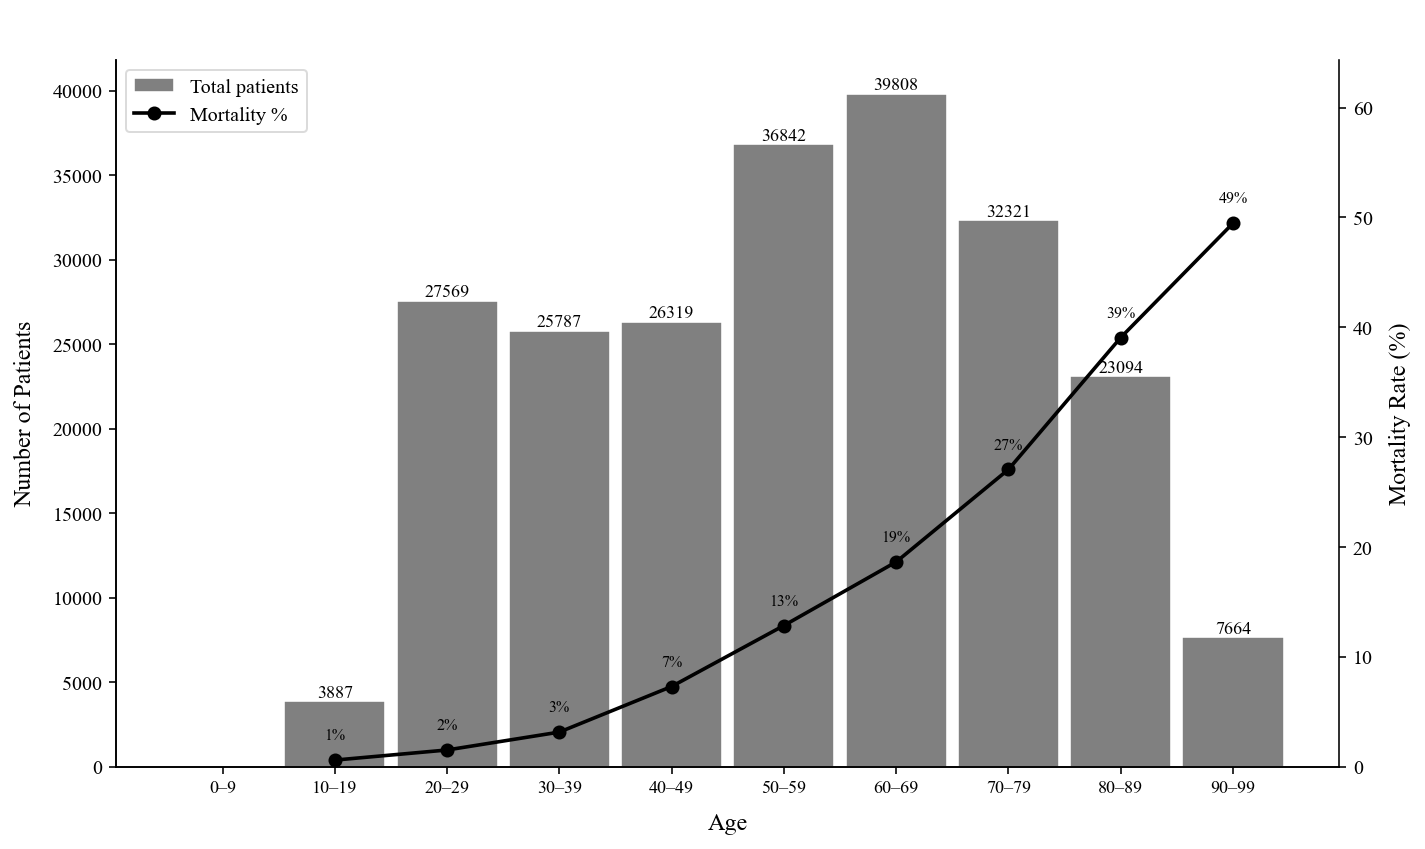
\includegraphics[width=0.9\textwidth]{hist2.png}
%     \caption{Age Distribution and Mortality Rates Among Patients in Our Dataset}
%     \label{fig.age_hist}
% \end{figure}

% In the dataset, patient ages range from 18 to 91 with an average of 56, and approximately 
% 54\% of patients are younger than 60. Patient ages are derived from the 
% \texttt{anchor\_age} column in \texttt{patients.csv}, which caps all ages above 89 at 
% 91~\citep{mimiciv}. Since our threshold of 60 falls below this ceiling, the cap does not 
% affect the analysis. The age distribution and mortality rates by age group are shown in 
% Figure~\ref{fig.age_hist}, using bins $[0,9],[10,19],\ldots,[80,89],[90,99]$.

% We solve problem~\eqref{form:LBBF} with constraint~\eqref{eq:oldagecon} included in 
% $\calX$ using the hybrid LBBD algorithm. Constraint~\eqref{eq:zmuLB} is excluded rather 
% than adjusted, in keeping with our intent to minimize tailoring of the methodology in the 
% presence of the new constraint. Table~\ref{tab.Extension} in 
% Appendix~\ref{App:tableDeets} reports detailed results, summarized in 
% Table~\ref{tab.ExtensionSum}. All instances across all size groups are solved to 
% optimality (0\% gap). The addition of this constraint appears to make instances more 
% tractable compared to the unconstrained results in Table~\ref{tab.SumH}.

% \begin{table}[htb]
%  \small \centering
%   \caption{Summary of Results from the Hybrid LBBD Algorithm with Age-Based 
%   Side-Constraint}
%  \label{tab.ExtensionSum}
%  \begin{threeparttable}
% \begin{tabular}{rrrrrrrrr}
%  \toprule
% Size & \multicolumn{2}{c}{Time} & \multicolumn{2}{c}{\#Opt cuts} & 
% \multicolumn{2}{c}{\#Feas cuts} & \multicolumn{2}{c}{\#CBB cuts}\\
%  & Avg & Range & Avg & Range & Avg & Range & Avg & Range\\
% \midrule
% \numprint{1000} & $<1$ & [$<1$, $<1$] & 5 & [3, 7] & 0 & [0, 0] & 0 & [0, 0]\\
% \numprint{5000} & 0 & [0, 1] & 55 & [35, 78] & 34 & [14, 56] & 0 & [0, 0]\\
% \numprint{10000} & 5 & [3, 9] & \numprint{228} & [\numprint{152}, \numprint{273}] & 
% \numprint{189} & [94, \numprint{277}] & 7 & [3, 13]\\
% \numprint{15000} & 36 & [12, 45] & \numprint{628} & [\numprint{359}, \numprint{742}] & 
% \numprint{595} & [\numprint{320}, \numprint{769}] & 81 & [27, \numprint{114}]\\
% \numprint{20000} & 113 & [89, \numprint{131}] & \numprint{1466} & [\numprint{1106}, 
% \numprint{1788}] & \numprint{1472} & [\numprint{948}, \numprint{1921}] & \numprint{290} & 
% [\numprint{224}, \numprint{350}]\\
% \numprint{25000} & \numprint{290} & [\numprint{226}, \numprint{397}] & \numprint{2724} & 
% [\numprint{2252}, \numprint{3537}] & \numprint{2836} & [\numprint{2101}, 
% \numprint{3848}] & \numprint{706} & [\numprint{511}, \numprint{992}]\\
% \numprint{30000} & 23 & [18, 29] & \numprint{584} & [\numprint{505}, \numprint{766}] & 
% \numprint{1015} & [\numprint{889}, \numprint{1322}] & 20 & [10, 31]\\
%  \bottomrule
% \end{tabular}
% \end{threeparttable}
% \end{table}

% Instances with \numprint{15000} patients or fewer are solved in under one minute, with the 
% \numprint{1000}-patient and \numprint{5000}-patient instances solved in under one second 
% using only optimality and feasibility cuts. For larger instances, CBB cuts are used more 
% frequently and running times remain within the time limit. For the \numprint{30000}-patient 
% instances, solution times range from 18 to 29 seconds.

% To examine the effect of the side constraint on the diseases identified, 
% Tables~\ref{tab.compa6025k} and~\ref{tab.compa6030k} report the cliques obtained with and 
% without constraint~\eqref{eq:oldagecon} for the \numprint{25000}-patient and 
% \numprint{30000}-patient samples, respectively. Results are presented column-wise for each 
% of the five samples, with ``W/O'' and ``W'' denoting solutions obtained without and with 
% the constraint, respectively. Each table reports the diseases in the clique alongside 
% their $a_{60}(\cdot)$ values, the mortality rate of the clique, and the average 
% $a_{60}(\cdot)$ across the clique. Tables~\ref{tab.a60_25k} and~\ref{tab.a60_30k} in 
% Appendix~\ref{App:tableDeets} summarize the $a_{60}$ values for all diseases appearing in 
% these tables across the two cohort sizes.

% \begin{table}[htb]
% \centering
% \caption{Optimal Solutions Found With and Without the Age-Based Side-Constraint on 
% \numprint{25000}-Patient Samples}
% \label{tab.compa6025k}
% \begin{threeparttable}
% \resizebox{\textwidth}{!}{
% \begin{tabular}{lr|lr|lr|lr|lr|lr|lr|lr|lr|lr}
% \toprule
% \multicolumn{4}{c|}{Sample \#1} & \multicolumn{4}{c|}{Sample \#2} & 
% \multicolumn{4}{c|}{Sample \#3} & \multicolumn{4}{c|}{Sample \#4} & 
% \multicolumn{4}{c}{Sample \#5} \\
% \midrule
% \multicolumn{2}{c|}{W/O} & \multicolumn{2}{c|}{W} & \multicolumn{2}{c|}{W/O} & 
% \multicolumn{2}{c|}{W} & \multicolumn{2}{c|}{W/O} & \multicolumn{2}{c|}{W} & 
% \multicolumn{2}{c|}{W/O} & \multicolumn{2}{c|}{W} & \multicolumn{2}{c|}{W/O} & 
% \multicolumn{2}{c}{W} \\
% \midrule
% Clique & $ a_{60} $ & Clique & $ a_{60} $ & Clique & $ a_{60} $ & Clique & $ a_{60} $ & 
% Clique & $ a_{60} $ & Clique & $ a_{60} $ & Clique & $ a_{60} $ & Clique & $ a_{60} $ & 
% Clique & $ a_{60} $ & Clique & $ a_{60} $ \\
% \midrule
% OACE & 0.72 & RCU & 0.56 & CA & 0.79 & ONSD & 0.56 & NCD & 0.88 & PIA & 0.48 & OACE & 
% 0.71 & Hepatitis & 0.28 & SEPT & 0.61 & DCP & 0.58 \\
% RF & 0.66 & FevUO & 0.44 & OACE & 0.72 & IntI & 0.54 & OACE & 0.72 & OLD & 0.47 & HF & 
% 0.79 & OLD & 0.47 & OACE & 0.72 & AlcD & 0.22 \\
% PNA & 0.63 & OLD & 0.48 & DLM & 0.73 & MD & 0.38 & AURF & 0.68 & & & PDX-Unacc & 0.50 & 
% ARenF & 0.71 & DLM & 0.73 & OLD & 0.48 \\
% OSNSD & 0.68 & & & RF & 0.66 & & & PDX-Unacc & 0.51 & & & SHK & 0.68 & & & PDX-Unacc & 
% 0.50 & ARenF & 0.71 \\
% PDX-Unacc & 0.51 & & & HF & 0.79 & & & OSNSD & 0.67 & & & FED & 0.61 & & & CoagHD & 
% 0.60 & & \\
%  &  &  &  & PDX-Unacc & 0.51 &  &  &  &  &  &  &  &  &  &  &  &  &  &  \\
% \midrule
% $ \mu $ & Avg & $ \mu $ & Avg & $ \mu $ & Avg & $ \mu $ & Avg & $ \mu $ & Avg & $ \mu $ 
% & Avg & $ \mu $ & Avg & $ \mu $ & Avg & $ \mu $ & Avg & $ \mu $ & Avg \\
% 0.97 & 0.64 & 0.68 & 0.49 & 0.97 & 0.70 & 0.67 & 0.49 & 0.98 & 0.69 & 0.69 & 0.48 & 
% 0.97 & 0.66 & 0.68 & 0.49 & 0.98 & 0.63 & 0.70 & 0.50 \\
% \bottomrule
% \end{tabular}
% }
% \begin{tablenotes}[flushleft]
% \item \scriptsize Disease names are abbreviated due to space limitations; full names are 
% provided in Appendix~\ref{App:abb}.
% \end{tablenotes}
% \end{threeparttable}
% \end{table}

% \begin{table}[htb]
% \centering
% \caption{Optimal Solutions Found With and Without the Age-Based Side-Constraint on 
% \numprint{30000}-Patient Samples}
% \label{tab.compa6030k}
% \begin{threeparttable}
% \resizebox{\textwidth}{!}{
% \begin{tabular}{lr|lr|lr|lr|lr|lr|lr|lr|lr|lr}
% \toprule
% \multicolumn{4}{c|}{Sample \#1} & \multicolumn{4}{c|}{Sample \#2} & 
% \multicolumn{4}{c|}{Sample \#3} & \multicolumn{4}{c|}{Sample \#4} & 
% \multicolumn{4}{c}{Sample \#5} \\
% \midrule
% \multicolumn{2}{c|}{W/O} & \multicolumn{2}{c|}{W} & \multicolumn{2}{c|}{W/O} & 
% \multicolumn{2}{c|}{W} & \multicolumn{2}{c|}{W/O} & \multicolumn{2}{c|}{W} & 
% \multicolumn{2}{c|}{W/O} & \multicolumn{2}{c|}{W} & \multicolumn{2}{c|}{W/O} & 
% \multicolumn{2}{c}{W} \\
% \midrule
% Clique & $ a_{60} $ & Clique & $ a_{60} $ & Clique & $ a_{60} $ & Clique & $ a_{60} $ & 
% Clique & $ a_{60} $ & Clique & $ a_{60} $ & Clique & $ a_{60} $ & Clique & $ a_{60} $ & 
% Clique & $ a_{60} $ & Clique & $ a_{60} $ \\
% \midrule
% HCSH & 0.79 & RCU & 0.55 & CHF-NH & 0.82 & AlcD & 0.20 & DOA & 0.59 & PS & 0.49 & 
% CardArr & 0.79 & AlcD & 0.21 & HCSH & 0.80 & AlcD & 0.21 \\
% ARF  & 0.62 & DOA & 0.59 & DOA    & 0.57 & OLD  & 0.50 & CardArr & 0.79 &      &      & 
% HCSH    & 0.79 & OLD  & 0.51 & SHK  & 0.68 & OLD  & 0.50 \\
% ONSD & 0.56 & AlcD & 0.22 & CUS    & 0.74 &      &      & GD      & 0.59 &      &      & 
% CHF-NH  & 0.82 &      &      & OA   & 0.62 &      &      \\
% RCU  & 0.55 &      &      &        &      &      &      & RCU     & 0.57 &      &      & 
% CUS     & 0.73 &      &      &      &      &      &      \\
%      &      &      &      &        &      &      &      & CA      & 0.81 &      &      &  
% &      &      &      &      &      &      &      \\
% \midrule
% $ \mu $ & Avg & $ \mu $ & Avg & $ \mu $ & Avg & $ \mu $ & Avg & $ \mu $ & Avg & $ \mu $ 
% & Avg & $ \mu $ & Avg & $ \mu $ & Avg & $ \mu $ & Avg & $ \mu $ & Avg \\
% 0.83 & 0.63 & 0.60 & 0.45 & 0.88 & 0.71 & 0.65 & 0.35 & 0.87 & 0.67 & 0.61 & 0.49 & 
% 0.84 & 0.78 & 0.66 & 0.36 & 0.85 & 0.70 & 0.64 & 0.36 \\
% \bottomrule
% \end{tabular}
% }
% \begin{tablenotes}[flushleft]
% \item \scriptsize Disease names are abbreviated due to space limitations; full names are 
% provided in Appendix~\ref{App:abb}.
% \end{tablenotes}
% \end{threeparttable}
% \end{table}

% The solutions obtained without the side constraint show a consistent pattern: every 
% disease in these cliques has $a_{60}(v) \ge 0.5$, meaning the majority of its patients are 
% aged 60 or older. For the \numprint{25000}-patient instances, diseases appearing in the 
% optimal cliques include neurocognitive disorders ($a_{60} = 0.88$), congestive heart 
% failure ($a_{60} = 0.79$), coronary atherosclerosis ($a_{60} = 0.79$), disorders of lipid 
% metabolism ($a_{60} = 0.73$), and other aftercare encounters ($a_{60} = 0.72$). The 
% \numprint{30000}-patient instances show a similar pattern, with congestive heart failure 
% ($a_{60} = 0.82$), hypertension with complications ($a_{60} = 0.80$), coronary 
% atherosclerosis ($a_{60} = 0.81$), and cardiac arrhythmia ($a_{60} = 0.79$) appearing 
% prominently. The average $a_{60}(\cdot)$ value across clique diseases exceeds 0.6 in all 
% instances, with mortality rates in the range $[0.97, 0.98]$ for the \numprint{25000}-patient 
% instances and $[0.83, 0.88]$ for the \numprint{30000}-patient instances. These results 
% indicate that, without the side constraint, the optimal cliques may reflect the elevated 
% baseline mortality of older patients as much as the synergistic lethality of co-occurring 
% diseases.

% The solutions obtained with the side constraint incorporate diseases with lower 
% $a_{60}(\cdot)$ values, including alcohol-related disorders ($a_{60} = 0.22$), hepatitis 
% ($a_{60} = 0.28$), mood disorders ($a_{60} = 0.38$), and fever of unknown origin 
% ($a_{60} = 0.46$). Mortality rates remain relatively high at $[0.67, 0.70]$ for the 
% \numprint{25000}-patient instances and $[0.60, 0.66]$ for the \numprint{30000}-patient 
% instances. In the presence of the age-based constraint, the high-mortality cliques 
% identified frequently include alcohol-related disorders, other liver diseases, and acute 
% renal failure. This observation is consistent with patterns reported in prior clinical 
% studies noting that alcohol-related liver disease co-occurring with acute kidney injury is 
% associated with elevated short-term mortality across adult age 
% ranges~\citep{altamirano2012acute}.

% The results of this case study illustrate that the hybrid LBBD framework accommodates 
% side constraints without modification to the core algorithm, and that the resulting 
% formulation remains tractable in practice.

% The next chapter concludes the dissertation by summarizing the contributions of this work, 
% discussing its limitations, and outlining directions for future research.

% \section{Enumeration and Exploring the Comorbidity Graph}

% To explore the comorbidity graph, we impose an explicit upper bound on the clique size. 
% Specifically, we restrict attention to $\ell$-frequent cliques whose cardinality does not exceed a prescribed integer $b$. 
% This restricted version aims to identify relatively small but highly lethal disease clusters in the comorbidity graph $G$, which may be particularly useful for clinicians assessing mortality risk in patients with multiple comorbidities. 
% From an algorithmic perspective, the bound on clique size also permits the use of effective enumerative approaches.

% The difference between the unrestricted version of the problem~\ref{eq.MMRCP} introduced in Chapter~\ref{sec.probstmnt}, where no bound is imposed on the size of the clique and the application we introduce in this section is that problem~\ref{eq.MMRCP} motivated by medical research applications, where restricting attention to small cliques may fail to capture broader interactions among comorbid diseases that jointly influence patient outcomes.

% Given positive integers  $b$, our problem of interest is to find an $\ell$-frequent clique $C$ in $G$  with at most $b$ diseases, for which the mortality rate $\mu(C)$ is a maximum. That is, we aim to solve the following optimization problem:
% \begin{equation}
%     \label{eq.MRP}\max\left\{\mu(C) : C \text{ is a non-empty $\ell$-frequent
%         clique in } G, |C| \le b\right\}.
% \end{equation}
% The upper-bound $b$ on clique size ensures that we identify smaller clusters associated with elevated mortality rates, as they hold greater diagnostic significance. It is usually the case that the mortality rates are higher for patients that have a large number of comorbidities. The lower-bound $\ell$ on the number of patients simultaneously afflicted with all diseases in $C$  ensures that the calculated mortality rate $\mu(C)$ is a reliable and indicative estimate from this dataset.  

% A variant of problem~\eqref{eq.MRP} is to identify a maximum \textit{marginal} mortality rate clique. Given a clique of diseases, we are interested  in identifying   diseases, the addition of which maximizes the overall mortality rate of the new clique. This further enhances the prognosis potential of this methodology for patient populations already afflicted with some diseases. Specifically, given a pre-established clique of strictly fewer than $b$ diseases denoted by $C^0$, we aim to identify at most $b-|C^0|$ additional disease(s) that maintain the clique property when added to $C^0$ and maximize the mortality rate of the new clique. That is, we now aim to solve the following optimization problem:
% \begin{equation}
%     \label{eq.margMRP}\max\left\{\mu(C) : C \text{ is a non-empty $\ell$-frequent
%         clique in } G, C \supseteq C^0, |C| \le b \right\}.
% \end{equation}
% It is easy to see that the maximum marginal mortality rate clique problem~\eqref{eq.margMRP} includes optimization problem~\eqref{eq.MRP} as a special case, obtained when $C^0 = \emptyset$ and both are special cases of problem~\ref{eq.MMRCP}.  


% % The following algorithm should be removed as it is moved to appendix.
% \begin{algorithm}[!htbp]
%     \KwIn{$\langle P, \widetilde{P}, A, G=(V,E), \ell, b\rangle$ and initial clique $C^0$ (possibly empty) such that $|C^0| < b$} 
%     \KwOut{Max-heap $\texttt{Q}$ of feasible cliques with mortality rate as priority}
%     $\texttt{Q} \gets \emptyset$\\
%     \If{$C^0\ne\emptyset$}{Insert $C^0$ in $\texttt{Q}$ with priority $\mu(C^0)$\\
%     $C \gets C^0$, $L \gets \bigcap\limits_{u \in C^0}N(u)$, and $\texttt{Den} \gets \bigcap\limits_{u \in C^0} A_u$}
%     \Else{$C \gets \emptyset$, $L \gets V$, and $\texttt{Den} \gets P$}
%     \SetKwFunction{FBronKerbosch}{Bron-Kerbosch}
%     \FBronKerbosch{$C,L,\texttt{Den}$}\\
%     \KwRet{$\texttt{Q}$}\\

%     \SetKwProg{Fn}{Function}{}{}
%     \Fn{\FBronKerbosch{$C,L,\texttt{Den}$}}{
%      \If{$|C|=b$ \text{or} $L = \emptyset$   \label{step.terminate} } {\KwRet}
%         \For{$v \in L$ \label{step.outer-for}}{
%             $\texttt{NewDen} \gets \texttt{Den} \cap A_v$\\
%             \If{$|\texttt{NewDen}| \ge \ell$}{
%                 $\mu \gets \frac{|\widetilde{P} \cap \texttt{NewDen}|}{|\texttt{NewDen}|}$\\
%                 $C \gets C \cup \{v\}$\\
%                 \If{$C \notin \texttt{Q}$}{
%                 Insert $C$ in $\texttt{Q}$ with priority $\mu$\\
%                 }
%                 \FBronKerbosch{$C, L\cap N(v),  \texttt{NewDen}$}\\
%             }
%             $L \gets L \setminus \{v\}$\\
%         }
%         \KwRet %$Q$
%     }
% \caption{Enumerating Highest (Marginal) Mortality Rate Cliques}
% \label{alg.BKMMRC}
% \end{algorithm}

% \hl{You can reduce the following explanation by refering and comparing this algorithm to the one in methodologies chapter which is commented next. Delete the commented part after being used.}

% % \begin{algorithm}[htbp]
% %     \SetKwFunction{FBronKerbosch}{Bron-Kerbosch}
% %     \SetKwProg{Fn}{Function}{}{}
% %     \KwIn{$\langle P, \widetilde{P}, A, G=(V,E), \ell\rangle$ and
% %     initial clique $C^0$ (possibly empty)}
% %     \KwOut{An $\ell$-frequent clique containing $C^0$ with maximum
% %     mortality rate}
% %     Initialize global variables $\texttt{BestSol} \gets C^0,\
% %     \texttt{BestObj} \gets \mu(C^0)$\\
% %     \If{$C^0 = \emptyset$}{
% %         $v \gets \arg\max_{u \in V} \mu(u)$\\
% %         $\texttt{BestSol} \gets \{v\},\ \texttt{BestObj} \gets
% %         \mu(v)$\\
% %         \FBronKerbosch{$\emptyset, V, P, \widetilde{P}$}
% %     }
% %     \Else{
% %         $L \gets \bigcap\limits_{u \in C^0} N(u) \setminus C^0$\\
% %         \FBronKerbosch{$C^0, L, \den(C^0), \num(C^0)$}
% %     }
% %     \KwRet{$\texttt{BestSol}$ and $\texttt{BestObj}$}\\
% %     \Fn{\FBronKerbosch{$C, L, \texttt{CurrentDen},
% %     \texttt{CurrentNum}$}}{
% %         \If{$L = \emptyset$ \label{step.terminate}}{\KwRet}
% %         \For{$v \in L$ \label{step.outer-for}}{
% %             $\texttt{NewDen} \gets \texttt{CurrentDen} \cap A_v$\\
% %             $\texttt{NewNum} \gets \texttt{CurrentNum} \cap A_v$\\
% %             \If{$|\texttt{NewDen}| \ge \ell$}{
% %                 \If{$\frac{|\texttt{NewNum}|}{|\texttt{NewDen}|} >
% %                 \texttt{BestObj}$}{
% %                     $\texttt{BestObj} \gets
% %                     \frac{|\texttt{NewNum}|}{|\texttt{NewDen}|}$\\
% %                     $\texttt{BestSol} \gets C \cup \{v\}$\\
% %                 }
% %                 \FBronKerbosch{$C \cup \{v\}, L \cap N(v),
% %                 \texttt{NewDen}, \texttt{NewNum}$}\\
% %             }
% %             $L \gets L \setminus \{v\}$\\
% %         }
% %         \KwRet
% %     }
% % \caption{Modified \footnotesize{Bron--Kerbosch} for the Maximum
% % Mortality Rate Clique Problem}
% % \label{alg.BKMMRC}
% % \end{algorithm}

% % Algorithm~\ref{alg.BKMMRC} solves MMRCP~\eqref{eq.MMRCP} and includes
% % a pruning step based on the following feasibility condition: a branch
% % is discarded whenever $\left|\bigcap_{u \in C} A_u\right| < \ell$,
% % i.e., whenever the current partial clique is not $\ell$-frequent. The
% % notation $N(v) \coloneqq \{u : \{u,v\} \in E\}$ denotes the
% % neighborhood of vertex $v$ in $G$.

% % Global variables \texttt{BestSol} and \texttt{BestObj} track the
% % incumbent clique and its mortality rate throughout the search, and are
% % updated whenever a feasible clique with a strictly higher mortality
% % rate is encountered. If $C^0$ is nonempty, it initializes the
% % incumbent; otherwise, the single-vertex clique with the highest
% % mortality rate serves as the initial incumbent. The candidate set $L$
% % is initialized to the common neighbors of all vertices in $C^0$ (or
% % all of $V$ if $C^0$ is empty), and \texttt{CurrentDen} and
% % \texttt{CurrentNum} are initialized to $\den(C^0)$ and $\num(C^0)$,
% % respectively (or $P$ and $\widetilde{P}$ if $C^0$ is empty). Because
% % these sets are passed as arguments and updated incrementally as $C$
% % grows, redundant recomputation is avoided.

% % The recursion terminates when $L$ is empty
% % (Step~\ref{step.terminate}), indicating that the current clique is
% % maximal. In each iteration of the for-loop, a vertex $v \in L$ is
% % considered for addition to $C$. The sets \texttt{NewDen} and
% % \texttt{NewNum} are computed and the $\ell$-frequency condition is
% % checked. If satisfied, the incumbent is updated whenever the mortality
% % rate of $C \cup \{v\}$ strictly exceeds \texttt{BestObj}, and a
% % deeper recursive call is made with the updated sets. Regardless of
% % whether $v$ is added, it is removed from $L$ after its recursive call
% % completes. Once all recursive calls are exhausted, \texttt{BestSol}
% % and \texttt{BestObj} contain the optimal solution to
% % MMRCP~\eqref{eq.MMRCP}.

% With a few simple tweaks in Algorithm~\ref{alg.BKMMRC}, we can achieve Algorithm~\ref{alg.BKMMRC} in Appendix~\ref{App:Pseudos} to solve both problems~\eqref{eq.MRP} and~\eqref{eq.margMRP}, which includes pruning steps based on the following feasibility conditions: \textit{(i)}~restricting the enumeration to cliques of size at most $b$, and \textit{(ii)}~eliminating  cliques associated with insufficient patients by enforcing that $\left|\bigcap\limits_{u \in C} A_u\right| \ge \ell$. 

% In Algorithm~\ref{alg.BKMMRC}, a global max-heap $Q$, prioritized by mortality rate, is used to store the enumerated cliques and if non-empty, $C^0$ is inserted in $Q$ initially. The disjoint sets $C$ and $L$ along with the set $den$, which represents the set $\bigcap\limits_{u \in C} A_u$ from the denominator of the mortality rate function are initialized next. Due to the recursive nature of the algorithm, it is more efficient to track and incrementally update $den$, rather than recompute the intersection of several sets every time. The current clique $C$ is initialized to $C^0$, the candidate set $L$ is initialized to the common neighbors of all the vertices in $C^0$ (or the entire vertex set if $C^0$ is empty), and $den$ is initialized to the set of patients that have all diseases in $C^0$ (or the entire patient set if $C^0$ is empty). 

%  Our algorithm terminates the recursion if one of the following conditions is met in Step~\ref{step.terminate} of Algorithm~\ref{alg.BKMMRC}: \textit{(i)}~when  $L$ is empty, which means that the current clique is maximal; or \textit{(ii)}~the size of current clique is $b$. As a clique is enlarged with the addition of a vertex $v$ in a recursive call, the set $den$ is updated, lower bound condition checked and if met, mortality rate is calculated. The new clique is inserted in $Q$ with its mortality rate as priority  if it is not already in the max-heap. Then a deeper recursive call is made with the updated sets. If candidate vertex $v \in L$ cannot be included due to the lower-bound $\ell$ not being satisfied, or if we added vertex $v$ and completed that recursive call,  vertex $v$ is removed from the set $L$. After the recursive calls are exhausted, the max-heap $Q$ contains all feasible cliques encountered, with their associated mortality rate as heap priority. We can now extract the clique with the highest (marginal) mortality rate and solve problems~\eqref{eq.MRP} and~\eqref{eq.margMRP}. More importantly, we can now return for any positive integer $K$, the cliques with the $K$ highest mortality rates. 



% \subsection{Scalability of the Modified Bron--Kerbosch 
% Algorithm}\label{sec.exp2-BKscalability}

% The goal of this section is to evaluate the performance of the modified BK 
% algorithm on the complete MIMIC-IV dataset of \numprint{223291} distinct patient records, 
% which represents the scale at which the problem is most relevant in practice. 
% Table~\ref{tab:mimicXBK} presents the results for this full dataset. Column ``\#Dec'' 
% records the number of deceased patients, i.e., the numerator of the mortality rate, for 
% reference, and column ``\#RC'' records the number of recursive calls made by the 
% algorithm. For the experiments in this section, we report the top-5 most lethal cliques 
% for each value of the clique size upper-bound $b$.

% \begin{table}[!ht]
%     \caption{Top-5 most lethal cliques in the \numprint{223291}-patient dataset found by 
%     the modified BK algorithm.}
%     \label{tab:mimicXBK}
%     \small \centering
%     {\begin{tabular}{clrrrr}
%      \toprule
%           $b$ & Clique & \#Dec & $\mu$ & Time (s) & \#RC\\
%           \midrule
%          \multirow{5}{*}{1} & OACE & \numprint{184636} & 0.83 & 
%          \multirow{5}{*}{\numprint{1}} & \multirow{5}{*}{\numprint{623}} \\
%           & CP & \numprint{172829} & 0.77 & & \\
%           & GCb & \numprint{165264} & 0.74 & & \\
%           & MNWo & \numprint{161972} & 0.73 & & \\
%           & ECP & \numprint{156766} & 0.70 & & \\
% \midrule
%      \multirow{5}{*}{2} & ECP, OACE & \numprint{211396} & 0.95 & 
%      \multirow{5}{*}{\numprint{4}} & \multirow{5}{*}{\numprint{9148}} \\
%           & HepF, OACE & \numprint{210706} & 0.94 & & \\
%           & AHCD, OACE & \numprint{207341} & 0.93 & & \\
%           & SHK, OACE & \numprint{206481} & 0.92 & & \\
%           & Coma, OACE & \numprint{206079} & 0.92 & & \\
% \midrule
%      \multirow{5}{*}{3} & ECP, CNTN, OACE & \numprint{214515} & 0.96 & 
%      \multirow{5}{*}{\numprint{24}} & \multirow{5}{*}{\numprint{136080}} \\
%           & ECP, SM, OACE & \numprint{213829} & 0.96 & & \\
%           & SHK, HepF, OACE & \numprint{213511} & 0.96 & & \\
%           & CD, HepF, OACE & \numprint{213124} & 0.95 & & \\
%           & RF, HepF, OACE & \numprint{213076} & 0.95 & & \\
% \midrule
%      \multirow{5}{*}{4} & SHK, HepF, UTI, OACE & \numprint{218016} & 0.98 & 
%      \multirow{5}{*}{\numprint{119}} & \multirow{5}{*}{\numprint{1570449}} \\
%           & CD, HepF, UTI, OACE & \numprint{217156} & 0.97 & & \\
%           & HP, AMI, OACE, DMWC & \numprint{216818} & 0.97 & & \\
%           & HF, HepF, OACE, PNA & \numprint{216799} & 0.97 & & \\
%           & HF, Hypo, HepF, OACE & \numprint{216524} & 0.97 & & \\
%          \bottomrule
%     \end{tabular}}
% \end{table}

% The modified BK algorithm handles the full dataset efficiently across all values of $b$. 
% Running time grows from 1 second at $b=1$ to 119 seconds at $b=4$, while the number of 
% recursive calls grows from 623 to over 1.5 million, reflecting the increasing 
% combinatorial complexity with clique size. Among individual diseases, other aftercare 
% encounter (OACE) has the highest mortality rate at 0.83, followed by cancer of pancreas 
% (CP) at 0.77 and gastrointestinal cancers of the bile duct (GCb) at 0.74. As expected, 
% the maximum mortality rate increases as $b$ grows from 1 to 4. At $b=2$, pairing ECP 
% with OACE yields the highest rate of 0.95; at $b=3$, the triple \{ECP, CNTN, OACE\} 
% reaches 0.96; and at $b=4$, the combination \{SHK, HepF, UTI, OACE\} attains 0.98. The 
% persistent appearance of OACE across all clique sizes at $b \ge 2$ reflects its frequent 
% co-occurrence with severe inpatient conditions in the MIMIC-IV dataset. The high mortality 
% rates associated with hepatic failure (HepF) in combination with shock (SHK) or cardiac 
% dysrhythmias (CD) are consistent with clinical observations of poor prognosis in patients 
% with acute-on-chronic liver failure and hemodynamic 
% instability~\citep{Hernaez2017,Moreau2013}. The recurrence of cancer-related groups (ECP, 
% CNTN, SM) is in line with the elevated short-term mortality documented in oncology 
% inpatients with advanced disease~\citep{Earle2008,Numico2015}.

% Our results reinforce clinical insights through large-scale EHR analysis. The absence of 
% spurious comorbidities among the highest mortality rate cliques is encouraging, as 
% spurious detections are a recognized concern in graph-based data mining. The data 
% preparation procedure and the structure of the modified BK algorithm together provide a 
% practically sound framework for comorbidity-based mortality analysis.

% In order to explore a broader set of disease interactions, we remove from the 
% \numprint{223291}-patient dataset every patient diagnosed with hepatic failure (HepF) or 
% other aftercare encounter (OACE), the two conditions most dominant in 
% Table~\ref{tab:mimicXBK}. The resulting cohort of \numprint{211391} patients is analyzed 
% using the modified BK algorithm, and results are reported in 
% Table~\ref{tab:mimicXBKdeletion}.

% \begin{table}[!ht]
%     \caption{Top-5 most lethal cliques in the \numprint{211391}-patient dataset found by 
%     the modified BK algorithm.}
%     \label{tab:mimicXBKdeletion}
%     \small \centering
%     {\begin{tabular}{clrrrr}
%           \toprule
%          $b$ & Clique & \#Dec & $\mu$ & Time (s)& \#RC\\[0.5ex]
%           \midrule
%          \multirow{5}{*}{1} & CP & \numprint{163619} & 0.77 & 
%          \multirow{5}{*}{\numprint{1}} & \multirow{5}{*}{\numprint{621}} \\
%           & GCb & \numprint{156457} & 0.74 & & \\
%           & MNWo & \numprint{153340} & 0.73 & & \\
%           & ECP & \numprint{148411} & 0.70 & & \\
%           & SM & \numprint{147450} & 0.70 & & \\
% \midrule
%      \multirow{5}{*}{2} & CAVF, Coma & \numprint{187321} & 0.89 & 
%      \multirow{5}{*}{\numprint{4}} & \multirow{5}{*}{\numprint{9018}} \\
%           & ARF, SM & \numprint{180327} & 0.85 & & \\
%           & ECP, CNTN & \numprint{179863} & 0.85 & & \\
%           & ECP, SM & \numprint{176676} & 0.84 & & \\
%           & RF, SM & \numprint{176562} & 0.84 & & \\
% \midrule
%      \multirow{5}{*}{3} & SM, ARF, PHD & \numprint{192554} & 0.91 & 
%      \multirow{5}{*}{\numprint{23}} & \multirow{5}{*}{\numprint{132907}} \\
%           & RF, CNTN, SM & \numprint{190924} & 0.90 & & \\
%           & ARF, SM, Phleb & \numprint{190876} & 0.90 & & \\
%           & SM, ND, PHD & \numprint{190640} & 0.90 & & \\
%           & CAVF, Coma, RF & \numprint{190251} & 0.90 & & \\
% \midrule
%       \multirow{5}{*}{4} & SHMSA, SM, ARF, PHD & \numprint{199754} & 0.94 & 
%       \multirow{5}{*}{\numprint{118}} & \multirow{5}{*}{\numprint{1523191}} \\
%           & RC, CNTN, RF, DLM & \numprint{199739} & 0.94 & & \\
%           & ARF, SHMSA, SM, Phleb & \numprint{199647} & 0.94 & & \\
%           & InjE, SM, DMWC, ARF & \numprint{199647} & 0.94 & & \\
%           & CoagHD, NV, PNA, SM & \numprint{198850} & 0.94 & & \\
%          \bottomrule
%     \end{tabular}}
% \end{table}

% After the exclusion, cancer of pancreas (CP) carries the highest individual mortality 
% rate at 0.77, followed by GCb at 0.74 and MNWo at 0.73. At $b=2$, the pair \{CAVF, 
% Coma\} achieves the highest pairwise rate of 0.89. Secondary malignancies (SM) feature 
% prominently across $b \in \{2,3,4\}$, appearing in the majority of top cliques at each 
% level. At $b=3$, the triple \{SM, ARF, PHD\} reaches a rate of 0.91, and at $b=4$, four 
% of the five top cliques achieve 0.94. Notably, the combination \{SHMSA, SM, ARF, PHD\} 
% at $b=4$ reaches 0.94, as does \{RC, CNTN, RF, DLM\}, which involves respiratory 
% cancers, cancer treatment-related conditions, respiratory failure, and lipid metabolism 
% disorders. The frequent co-occurrence of SM with pulmonary and hematologic conditions is 
% consistent with the elevated mortality observed in patients with multi-organ involvement 
% in advanced malignancy~\citep{Earle2008,Numico2015,Charlson1987}. The combination of 
% respiratory cancers with respiratory failure and metabolic derangement reflects 
% well-documented interactions between advanced cancer and systemic 
% compromise~\citep{Niederman2022}.

% Analyzing the dataset after removing the dominant diseases from Table~\ref{tab:mimicXBK} 
% reveals a qualitatively different set of lethal comorbidity patterns, illustrating how 
% the framework can be used to investigate lesser-known disease combinations. The rapid 
% escalation of mortality rates with increasing clique size, even among diseases not 
% individually recognized as acutely lethal, underscores the value of a systematic 
% comorbidity-aware approach.

% \subsection{Sensitivity Analysis and Marginal Mortality 
% Rates}\label{sec.exp3-margMR}

% The experiments in this section focus on problem~\eqref{eq.MMRCP} when $C^0$ is 
% non-empty. We use the \numprint{211391}-patient dataset from the previous section, which 
% excludes all patients diagnosed with hepatic failure or other aftercare encounter. For 
% each value of $b$, we set $C^0$ to be the fifth highest mortality rate clique from 
% Table~\ref{tab:mimicXBKdeletion}. This choice is deliberate: the results in 
% Tables~\ref{tab:mimicXBK} and~\ref{tab:mimicXBKdeletion} already exhibit a sequence of 
% containment relationships among the top cliques as $b$ increases, so fixing $C^0$ in 
% this way directs the search toward high marginal mortality rate cliques not immediately 
% visible from those tables.

% Two experiments are conducted for each $C^0$. (\textit{i})~For each $u \in V \setminus 
% C^0$, we compute $\mu(C^0 \cup \{u\})$ without requiring $C^0 \cup \{u\}$ to be a 
% clique, and return the top-3 highest marginal mortality rate subsets. 
% (\textit{ii})~Algorithm~\ref{alg.BKMMRC} is used to find the top-3 highest marginal 
% mortality rate \textit{cliques} containing $C^0$, allowing the addition of one and then 
% two more diseases.

% \begin{table}[!ht]
% \caption{Top-3 most lethal subsets formed by the addition of a single disease.}
% \label{tab:margMRplus1SA}
% \centering
% \resizebox{\textwidth}{!}{%
% \begin{tabular}{lclcrr}
% \toprule
% {Initial clique $C^0$} & \multicolumn{1}{c}{{$\mu(C^0)$}} & {Additional disease $u$} & 
% {$\mu(C^0 \cup \{u\})$} & {\%Increase} & Cluster type\\
% \midrule
% \multirow{5}{*}{SM} & 0.70 & Coma & 0.87 & 25.34\% & 1-defective clique \\
%  & 0.70 & APV & 0.86 & 23.56\% & 1-defective clique \\
%  & 0.70 & CUS & 0.86 & 22.7\% & 1-defective clique \\
%  & 0.70 & ARF & 0.85 & 22.3\% & clique \\
%  & 0.70 & SHK & 0.85 & 21.35\% & 1-defective clique \\
% \midrule
% \multirow{5}{*}{RF, SM} & 0.84 & ECP & 0.95 & 13.28\% & 1-defective clique\\
%  & 0.84 & DOA & 0.92 & 10.71\% & 2-defective clique \\
%  & 0.84 & OLRD & 0.92 & 9.99\% & 2-defective clique \\
%  & 0.84 & DSD & 0.91 & 9.46\% & 1-defective clique \\
%  & 0.84 & PF & 0.91 & 9.28\% & 1-defective clique \\
% \midrule
% \multirow{3}{*}{CAVF, Coma, RF} & 0.90 & AURF & 0.91 & 1.45\% & 1-defective clique\\
%  & 0.90 & FED & 0.91 & 0.6\% & clique \\
%  & 0.90 & PDX-Unacc & 0.90 & -0.2\% & 2-defective clique \\
% \midrule
% \multirow{2}{*}{CoagHD, NV, PNA, SM} & 0.94 & FED & 0.94 & 0.45\% & clique \\
%  & 0.94 & PDX-Unacc & 0.94 & 0\% & clique \\[3pt]
% \bottomrule
% \end{tabular}%
% }
% \end{table}

% Table~\ref{tab:margMRplus1SA} reports the results of experiment (\textit{i}). For each 
% $C^0$ in the first column, the additional disease $u$ yielding the highest, second 
% highest, and third highest increase in mortality rate is listed in the third column. The 
% column ``\%Increase'' records the percentage by which $\mu(C^0 \cup \{u\})$ exceeds 
% $\mu(C^0)$.

% When $C^0$ is small, $\mu(C^0)$ is relatively low and the addition of a single disease 
% can produce substantial gains. Adding coma to the singleton clique \{SM\} raises the 
% mortality rate from 0.70 to 0.87 (a 25.34\% increase), while adding aspiration 
% pneumonitis (APV) yields a 23.56\% increase. By contrast, when $|C^0|$ is larger and 
% $\mu(C^0)$ is already high, marginal gains diminish: for $C^0 = \{\text{CoagHD, NV, PNA, 
% SM}\}$ with $\mu(C^0) = 0.94$, no addition produces an increase exceeding 0.5\%. These 
% observations reinforce the focus on small but lethal cliques throughout this work and 
% justify restricting $b$ to at most 4 in the main experiments.

% A further observation concerns the structural types of the detected subsets, as reported 
% in the column ``Cluster type''. We characterize each subset using the notion of a 
% $k$-defective clique: a vertex set $S \subset V$ is $k$-defective if the induced subgraph 
% $G[S]$ contains at least $\binom{|S|}{2} - k$ edges, i.e., it falls short of a complete 
% graph by at most $k$ edges. A standard clique is 0-defective. This characterization is 
% used here as a natural way to describe near-clique structure; alternative relaxations 
% such as $k$-plexes~\citep{BBSBIVH11kplex} or $\gamma$-quasi-cliques~\citep{Pattillo2013qclique} 
% could also be applied with suitable parameter choices. Among the subsets in 
% Table~\ref{tab:margMRplus1SA}, 9 out of 12 are 0-defective or 1-defective cliques, 
% although a 2-vertex 1-defective clique amounts to two isolated vertices, which is not a 
% particularly informative cluster structure. Importantly, 9 out of 12 subsets induce 
% connected subgraphs; three representative examples are visualized in 
% Figure~\ref{fig.defclq123}.

% It is worth noting that an edge in the comorbidity graph reflects co-occurrence above the 
% threshold $\Delta$ in the EHR dataset. Accordingly, for two diseases $u, v \in V$, it is 
% possible that $\sigma(u,v) < \Delta$ while $|A_u \cap A_v| \ge \ell$, so a subset may 
% contain non-adjacent disease pairs and still correspond to a strictly positive mortality 
% rate. The choice of $\ell = 100$ used throughout is illustrative; larger values of $\ell$ 
% may yield different clusters.

% \begin{figure}[!ht]
%     \centering
%     \begin{tikzpicture}
%     [scale=.8,auto=left,every node/.style={circle, draw, black, fill=blue!20, 
%     minimum size = 2pt}]
%     \node (n1) at (-1,1){$u$};
%     \node (n2) at (-3.25,4)  {};
%     \node (n3) at (-3.25,2.5)  {};
%     \node (x1) at (4.5,1){$u$};
%     \node (x2) at (2.5,4)  {};
%     \node (x3) at (4.5,2.5)  {};
%     \node (x4) at (6.5,4)  {};
%     \node (c1) at (8,2.5){};
%     \node (c2) at (8,4)  {};
%     \node (c3) at (9,1)  {$u$};
%     \node (c4) at (10,2.5) {};
%     \node (c5) at (10,4)  {};
%     \foreach \from/\to in {n1/n3,n3/n2,
%     x1/x3,x2/x3,x2/x4,x3/x4,
%     c1/c2,c1/c3,c1/c4,c1/c5,c2/c3,c2/c4,c2/c5,c3/c4,c3/c5,c4/c5}
%     \draw[thick] (\from) -- (\to);
%     \end{tikzpicture}
%     \caption{From left to right, the subgraphs induced by the following subsets from 
%     Table~\ref{tab:margMRplus1SA}: 1-defective clique \{RF, SM, ECP ($u$)\}; 
%     2-defective clique \{CAVF, Coma, RF, PDX-Unacc ($u$)\}; clique \{CoagHD, NV, PNA, SM, 
%     FED ($u$)\}. The added vertex $u$ is labeled in each graph.}
%     \label{fig.defclq123}
% \end{figure}

% Our final experiments assess the performance of Algorithm~\ref{alg.BKMMRC} given a 
% non-empty $C^0$. The modified BK algorithm is well-suited to this setting and runs 
% extremely fast when initialized with an existing disease clique. 
% Tables~\ref{tab:margMRplus1t4} and~\ref{tab:margMRplus2t4} report results that are 
% complementary to those in Table~\ref{tab:mimicXBKdeletion} and exhibit trends consistent 
% with Table~\ref{tab:margMRplus1SA}. These results identify the diseases most consequential 
% to monitor when a patient already carries a known set of diagnoses, which is the primary 
% purpose of the marginal mortality rate analysis.

% \begin{table}[!ht]
% \caption{Top-3 most lethal cliques formed by the addition of a single disease.}
% \label{tab:margMRplus1t4}
% \centering
% \resizebox{\textwidth}{!}{%
% \begin{tabular}{lclcrrr}
% \toprule
% {$C^0$} & \multicolumn{1}{c}{{$\mu(C^0)$}} & {Additional disease $u$} & 
% {$\mu(C^0 \cup \{u\})$} & {\%Increase} & Time (s) & \#RC \\
% \midrule
% \multirow{3}{*}{SM} & 0.70 & ARF & 0.85 & 22\% & \multirow{3}{*}{\numprint{52}} & 
% \multirow{3}{*}{52} \\
%  & 0.70 & CP & 0.83 & 20\% & & \\
%  & 0.70 & PNAS & 0.83 & 19\% & & \\
% \midrule
% \multirow{3}{*}{RF, SM} & 0.84 & CNTN & 0.90 & 8\% & \multirow{3}{*}{\numprint{44}} & 
% \multirow{3}{*}{44} \\
%  & 0.84 & Aphleb & 0.89 & 7\% & & \\
%  & 0.84 & DKU & 0.89 & 6\% & & \\
% \midrule
% \multirow{1}{*}{CAVF, Coma, RF} & 0.90 & FED & 0.91 & 1\% & \multirow{1}{*}{\numprint{2}} 
% & \multirow{1}{*}{2} \\
% \midrule
% \multirow{2}{*}{CoagHD, NV, PNA, SM} & 0.94 & FED & 0.94 & 0\% & 
% \multirow{2}{*}{\numprint{3}} & \multirow{2}{*}{3} \\
%  & 0.94 & PDX-Unacc & 0.94 & 0\% & & \\[3pt]
% \bottomrule
% \end{tabular}%
% }
% \end{table}

% \begin{table}[!ht]
% \caption{Top-3 most lethal cliques formed by the addition of two diseases.}
% \label{tab:margMRplus2t4}
% \centering
% \resizebox{\textwidth}{!}{%
% \begin{tabular}{lclcrrr}
% \toprule
% {$C^0$} & \multicolumn{1}{c}{{$\mu(C^0)$}} & {Additional diseases $u,v$} & 
% {$\mu(C^0 \cup \{u,v\})$} & {\%Increase} & {Time (s)} & {\#RC} \\
% \midrule
% \multirow{3}{*}{SM} & 0.70 & SEPTL, PHD & 0.91 & 31\% & 
% \multirow{3}{*}{\numprint{787}} & \multirow{3}{*}{\numprint{787}} \\
%  & 0.70 & ARF, Phleb & 0.90 & 29\% & & \\
%  & 0.70 & ND, PHD & 0.90 & 29\% & & \\
% \midrule
% \multirow{3}{*}{RF, SM} & 0.84 & DKU, CNTN & 0.94 & 12\% & 
% \multirow{3}{*}{\numprint{748}} & \multirow{3}{*}{\numprint{748}} \\
%  & 0.84 & CNTN, GSS & 0.94 & 12\% & & \\
%  & 0.84 & CNTN, SEPT & 0.94 & 12\% & & \\
% \midrule
% \multirow{1}{*}{CAVF, Coma, RF} & 0.90 & FED & 0.91 & 1\% & 
% \multirow{1}{*}{\numprint{2}} & \multirow{1}{*}{2} \\
% \midrule
% \multirow{2}{*}{CoagHD, NV, PNA, SM} & 0.94 & FED, PDX-Unacc & 0.94 & 0\% & 
% \multirow{2}{*}{\numprint{4}} & \multirow{2}{*}{4} \\
%  & 0.94 & PDX-Unacc & 0.94 & 0\% & & \\[3pt]
% \bottomrule
% \end{tabular}%
% }
% \end{table}

% Table~\ref{tab:margMRplus1t4} shows that when $C^0 = \{\text{SM}\}$, adding adult 
% respiratory failure (ARF) yields the largest improvement, raising $\mu$ from 0.70 to 0.85 
% (22\%), followed by CP and pneumonia (PNAS) at 20\% and 19\% respectively. For $C^0 = 
% \{\text{RF, SM}\}$, adding conditions due to neoplasm or its treatment (CNTN) raises the 
% rate from 0.84 to 0.90 (8\%), with acute phlebitis (Aphleb) and diseases of kidney and 
% ureters (DKU) close behind. For larger cliques, the gains are marginal: both 
% \{CAVF, Coma, RF\} and \{CoagHD, NV, PNA, SM\} admit improvements of at most 1\% from 
% any single addition. Algorithm~\ref{alg.BKMMRC} completes all single-addition runs in at 
% most 52 seconds with at most 52 recursive calls, confirming its efficiency when 
% initialized with a non-empty $C^0$.

% Table~\ref{tab:margMRplus2t4} reports the results when two diseases are added 
% simultaneously. Larger gains are possible for smaller initial cliques: adding SEPTL and 
% PHD to \{SM\} raises the mortality rate to 0.91 (31\%), and adding DKU and CNTN to 
% \{RF, SM\} raises it to 0.94 (12\%). For the larger cliques, the maximum gain from any 
% two-disease addition remains at or below 1\%, consistent with the pattern observed in 
% Table~\ref{tab:margMRplus1t4}. All two-addition runs complete within 787 seconds and 787 
% recursive calls. Together, Tables~\ref{tab:margMRplus1t4} and~\ref{tab:margMRplus2t4} 
% demonstrate the utility of the framework for identifying which additional diseases pose 
% the greatest incremental risk for a patient already carrying a known set of diagnoses.

